\documentclass[journal]{vgtc}                % final (journal style)
%\documentclass[review,journal]{vgtc}         % review (journal style)
%\documentclass[widereview]{vgtc}             % wide-spaced review
%\documentclass[preprint,journal]{vgtc}       % preprint (journal style)
%\documentclass[electronic,journal]{vgtc}     % electronic version, journal

%% Uncomment one of the lines above depending on where your paper is
%% in the conference process. ``review'' and ``widereview'' are for review
%% submission, ``preprint'' is for pre-publication, and the final version
%% doesn't use a specific qualifier. Further, ``electronic'' includes
%% hyperreferences for more convenient online viewing.

%% Please use one of the ``review'' options in combination with the
%% assigned online id (see below) ONLY if your paper uses a double blind
%% review process. Some conferences, like IEEE Vis and InfoVis, have NOT
%% in the past.

%% Please note that the use of figures other than the optional teaser is not permitted on the first page
%% of the journal version.  Figures should begin on the second page and be
%% in CMYK or Grey scale format, otherwise, colour shifting may occur
%% during the printing process.  Papers submitted with figures other than the optional teaser on the
%% first page will be refused.

%% These three lines bring in essential packages: ``mathptmx'' for Type 1
%% typefaces, ``graphicx'' for inclusion of EPS figures. and ``times''
%% for proper handling of the times font family.

\usepackage{mathptmx}
\usepackage{graphicx}
\usepackage{times}

\usepackage{flushend}
\usepackage{subfigure}
\usepackage{amsmath}
\usepackage{amssymb}

\usepackage{vector}
\usepackage{algorithmic}
\usepackage{algorithm}

\renewcommand{\algorithmicrequire}{\textbf{Input:}}
\renewcommand{\algorithmicensure}{\textbf{Output:}}
\setlength\fboxsep{0pt}
\setlength\abovecaptionskip{0.18cm}

\usepackage{color}
\newcommand{\warn}[1]{{\color{red} [#1]}}
\newcommand{\todo}[1]{\textbf{\textcolor{blue}{[TODO: {#1}]}}}

%% We encourage the use of mathptmx for consistent usage of times font
%% throughout the proceedings. However, if you encounter conflicts
%% with other math-related packages, you may want to disable it.

%% This turns references into clickable hyperlinks.
\usepackage[bookmarks,backref=false,linkcolor=black]{hyperref} %,colorlinks
\hypersetup{
  pdfauthor = {},
  pdftitle = {},
  pdfsubject = {},
  pdfkeywords = {},
  colorlinks=true,
  linkcolor= black,
  citecolor= black,
  pageanchor=true,
  urlcolor = black,
  plainpages = false,
  linktocpage
}

%% If you are submitting a paper to a conference for review with a double
%% blind reviewing process, please replace the value ``0'' below with your
%% OnlineID. Otherwise, you may safely leave it at ``0''.
\onlineid{229}

%% declare the category of your paper, only shown in review mode
\vgtccategory{Algorithm/Technique}

%% allow for this line if you want the electronic option to work properly
\vgtcinsertpkg

%% In preprint mode you may define your own headline.
%\preprinttext{To appear in an IEEE VGTC sponsored conference.}

%% Paper title.

\title{Coherency-Based Curve Compression\\ for High-Order Finite Element Model Visualization}

%% This is how authors are specified in the journal style

%% indicate IEEE Member or Student Member in form indicated below
\author{Alexander Bock, Erik Sund\'en, Bingchen Liu,\\Burkhard W{\"u}nsche, \textit{Member, IEEE}, and Timo Ropinski, \textit{Member, IEEE}}
\authorfooter{
%% insert punctuation at end of each item
\item
 Alexander Bock,  Erik Sund\'en and Timo Ropinski are with the Scientific Visualization Group, Link\"oping University, Sweden, E-mail: \{alexander.bock, erik.sunden, timo.ropinski\}@liu.se.
\item
 Bingchen Liu and Burkhard W{\"u}nsche are with the Computer Science Department, University of Auckland, New Zealand, E-mail: \{bliu035, b.wuensche\}@auckland.ac.nz.
}

%other entries to be set up for journal
%\shortauthortitle{Biv \MakeLowercase{\textit{et al.}}: Global Illumination for Fun and Profit}
%\shortauthortitle{Firstauthor} \MakeLowercase{\textit{et al.}}: Paper Title


%% Abstract section.
\abstract{Finite element (FE) models are frequently used in engineering and life sciences within time-consuming simulations. In contrast with the regular grid structure facilitated by volumetric data sets, as used in medicine or geosciences, FE models are defined over a non-uniform grid. Elements can have curved faces and their interior can be defined through high-order basis functions, which pose additional challenges when visualizing these models. During ray-casting, the uniformly distributed sample points along each viewing ray must be transformed into the material space defined within each element. The computational complexity of this transformation makes a straightforward approach inadequate for interactive data exploration. In this paper, we introduce a novel coherency-based method which supports the interactive exploration of FE models by decoupling the expensive world-to-material space transformation from the rendering stage, thereby allowing it to be performed within a precomputation stage. Therefore, our approach computes view-independent proxy rays in material space, which are clustered to facilitate data reduction. During rendering, these proxy rays are accessed, and it becomes possible to visually analyze high-order FE models at interactive frame rates, even when they are time-varying or consist of multiple modalities. Within this paper, we provide the necessary background about the FE data, describe our decoupling method, and introduce our interactive rendering algorithm. Furthermore, we provide visual results and analyze the error introduced by the presented approach.} % end of abstract

%% Keywords that describe your work. Will show as 'Index Terms' in journal
%% please capitalize first letter and insert punctuation after last keyword
\keywords{Finite element visualization, GPU-based ray-casting.}

%% ACM Computing Classification System (CCS). 
%% See <http://www.acm.org/class/1998/> for details.
%% The ``\CCScat'' command takes four arguments.

\CCScatlist{ % not used in journal version
 \CCScat{I.3.7}{Computer Graphics}{Three-Dimensional Graphics and Realism}{Color, shading, shadowing, and texture}
}

%% Uncomment below to include a teaser figure.
\teaser{
	\centering 
  \subfigure{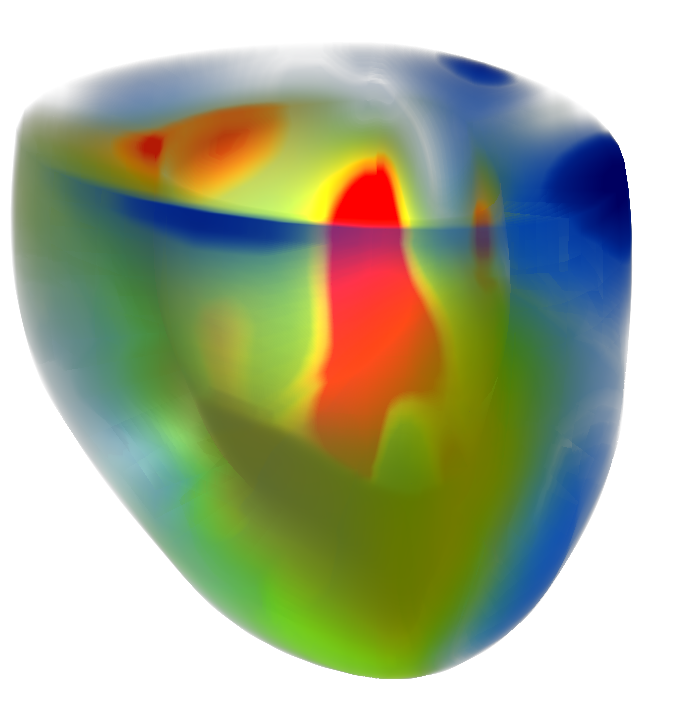
\includegraphics[width=0.22\linewidth]{figures/Heart1New1_T1}}
  \subfigure{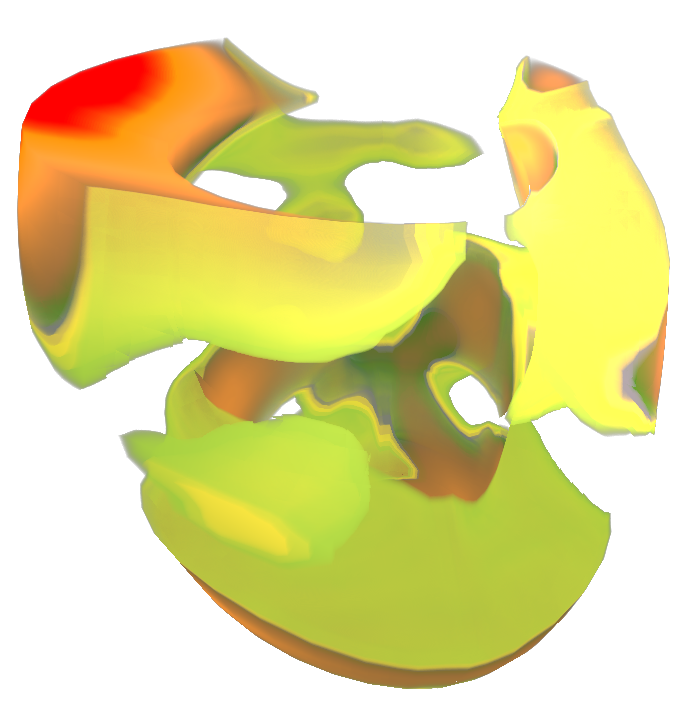
\includegraphics[width=0.22\linewidth]{figures/Heart1New2_T2}}
  \subfigure{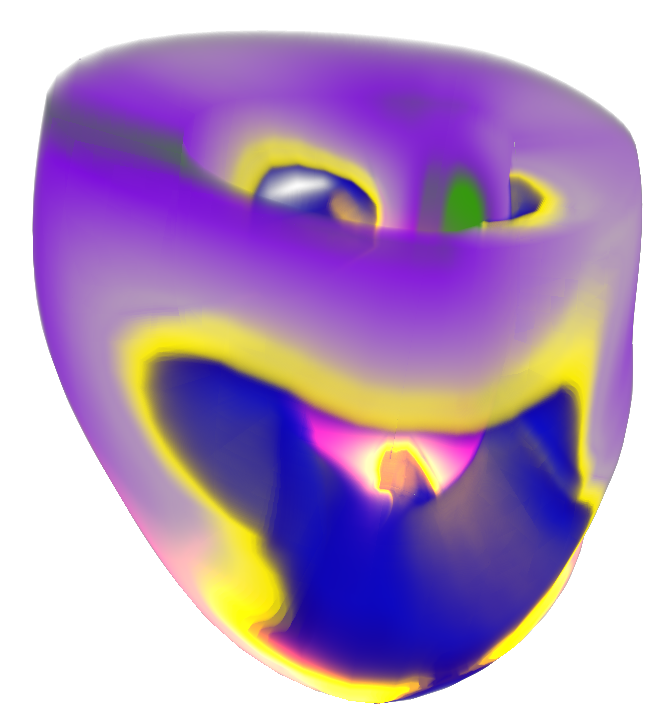
\includegraphics[width=0.22\linewidth]{figures/Heart4New1_T3}}
  \subfigure{\includegraphics[width=0.22\linewidth]{figures/HeartCombined}}
  \caption{Application of our visualization approach to a multi-parametric FE model of the left ventricle of a human heart. The images show volumetric renderings of different strain directions defined over the FE model: radial strain, circumferential strain, longitudinal strain as well as the three former combined ({\it left to right}). The presented approach allows for interactive data exploration by changing the transfer function and other relevant rendering parameters.}
  \label{fig:teaser}
}

%% Uncomment below to disable the manuscript note
%\renewcommand{\manuscriptnotetxt}{}

%% Copyright space is enabled by default as required by guidelines.
%% It is disabled by the 'review' option or via the following command:
% \nocopyrightspace

%%%%%%%%%%%%%%%%%%%%%%%%%%%%%%%%%%%%%%%%%%%%%%%%%%%%%%%%%%%%%%%%
%%%%%%%%%%%%%%%%%%%%%% START OF THE PAPER %%%%%%%%%%%%%%%%%%%%%%
%%%%%%%%%%%%%%%%%%%%%%%%%%%%%%%%%%%%%%%%%%%%%%%%%%%%%%%%%%%%%%%%%

\begin{document}
%
%% The ``\maketitle'' command must be the first command after the
%% ``\begin{document}'' command. It prepares and prints the title block.
%
%% the only exception to this rule is the \firstsection command
\firstsection{Introduction}\label{sec:introduction}
%
\maketitle
%
\begin{figure*}[t]
    \centering
    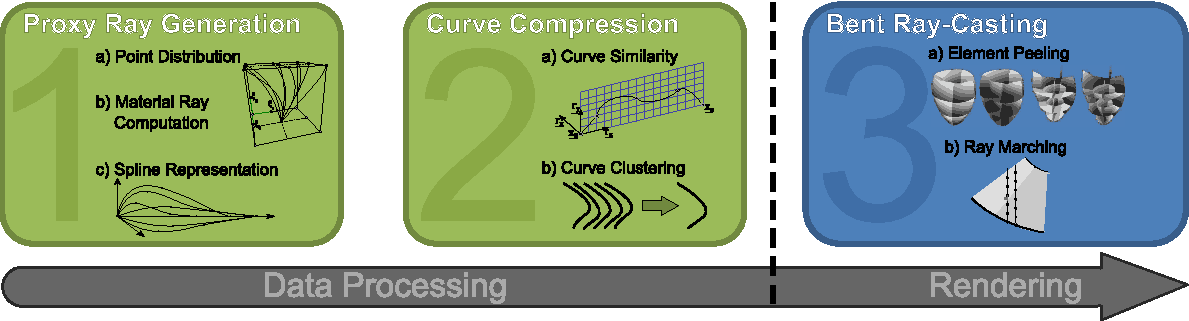
\includegraphics[width=0.85\textwidth]{figures/workflow-new.pdf}
    \caption{\textbf{Workflow.} To enable interactive ray-casting of curvilinear FE models, we exploit a multi-stage preprocessing approach. In the first step, we compute representative curved rays in material space, which are represented as splines and transformed in the second step into a common coordinate system. To reduce the amount of data for the subsequent rendering stage, we apply a rotation invariant curve clustering in the third step. The resulting data is then passed to the GPU-based rendering stage, where ray marching is performed.}
    \label{fig:workflow}
\end{figure*}
%
%
%
The finite element (FE) method is a computational technique frequently applied in science, medicine, and engineering to solve partial differential and integral equations~\cite{Young00}. The technique enables the discretization of complicated domains into arbitrarily shaped elements, in which material properties can be defined using nodal parameters together with potentially high-order interpolation functions. Thus, it becomes possible to incorporate material properties at every point rather than a limited number of sample points. Applications range from simulations of physical processes over derivation of new entities from measured data, for example,~computation of material strain from displacement data, to analyses and comparisons of data defined over objects with similar topology. All of these applications involve large amounts of multi-dimensional and multi-parametric data defined over arbitrary shaped grid structures. A prominent application example from bioengineering, in which FE visualization is essential, is the strain analysis of the human heart. An understanding of the full 3D strain tensor, represented by a symmetric matrix at each point, is necessary to identify unusual behavior of the heart muscle's deformation and to detect common patterns indicating developing diseases. Since there is little knowledge available about the exact behavior, interactive exploration plays an important role in the quest for new discoveries. By providing immediate visual feedback through rapid image generation, interactivity enables a rapid response to human input. In our case, it should be possible to interactively change all relevant visualization parameters, for example, parameter mapping and view orientation, such that the latency does not hinder the volumetric exploration process. While interactive surface-based visualizations of FE models are well established, volumetric visualization techniques supporting the interactive analysis of the entire structure are rare~\cite{Wihelms90}. This is largely due to the fact, that accessing the materials defined over high-order basis functions, which needs to be done for each sample in a volumetric visualization approach, involves high computational complexity.

In this paper, we introduce an interactive volumetric ray-casting algorithm for FE models that exploits ray coherency. When ray-casting FE models, viewing rays are straight lines in world space, but bent to curves in material (or $\xi$) space. Consequently, each sample point on a straight viewing ray must be transformed during rendering onto the corresponding curve in material space before the FE data can be fetched. To avoid this computationally complex transformation, we exploit ray coherency within a curve clustering approach, and thus precompute a view-independent proxy representation of the curved rays that can be accessed efficiently during rendering. The workflow of our approach is shown in Figure~\ref{fig:workflow}. In the first step we compute a representative subset of curved rays in material space, which are represented by splines. This subset is then reduced through clustering within the second curve compression step to obtain a lower number of curves, to which we refer as \emph{proxy rays}. Assuming that the proxy rays sufficiently represent the coherent curves of a FE model, we can access them in the third step, the rendering step, where we can omit the expensive world-to-material space transformation. This allows us to enable volumetric FE model visualization of potentially multi-parametric FE models on modern graphics processing units (GPUs) at interactive frame rates (see Figure~\ref{fig:teaser}). As we achieve this interactivity by exploiting preprocessing algorithms and data structures accessed during rendering. The costs of our approach are increased precomputation times as well as memory consumption, which are discussed in more detail in Sections~\ref{subsec:performance} and \ref{subsec:memory}. While our current implementation is constrained to hexahedral FE models, we will discuss the implications for other cell types within Section~\ref{subsec:limitations}.
%
%
%
\section{Related Work}\label{sec:relatedwork}
Interactive high-quality rendering of FE models, incorporating the interior of the elements, is a demanding task. Often, the elements are resampled to lie on a common regular uniform grid~\cite{Wihelms90}. While this enables a direct visualization using standard volume rendering algorithms, it also results in sampling-based errors as well as a loss of the easy access to element boundaries. As a consequence, many researchers have investigated rendering techniques that enable a more direct FE visualization by maintaining the relationship between the world and the material coordinate system.

W{\"u}nsche introduced an isosurface-based approach for the visualization of biomedical tensor field data~\cite{wunsche03femvis}, which has been applied to strain analysis. Another technique for rendering isosurfaces was presented by Nelson~et~al. in which they considered spectral high-order FE  meshes and introduced the idea of an error budget~\cite{nelsonhp06}. Schroeder~et~at. developed a framework for isosurface rendering by tessellating the basis functions into simpler forms which improves the mesh quality~\cite{schroeder06femtess}. Meyer~et~al. chose an approach based on particle systems to render isosurfaces efficiently~\cite{Meyer06}.

An alternative to the isosurface-based method was presented by Brasher~et~al.~\cite{brasher04} and Nelson~et~al.~\cite{nelson11}, in which cut planes through the high-order finite element data are evaluated. Rose and Ertl proposed a texture-based mesh reduction approach in order to render surface representations of large FE models at interactive frame rates~\cite{rose03femvis}. Other authors have proposed algorithms which exploit a conversion into a tetrahedral mesh representation~\cite{Reed95IncrementalSlicing, marmitt05femtess, Georgii06ageneric} which, in comparison with regular grid sampling, allow for adaptivity.

To improve rendering quality ray-casting approaches have been proposed. Garrity was one of the first to introduce ray-casting for rendering of unstructured meshes~\cite{garrity90RaytracingIrregular}. The technique is suitable for FE models as it tracks numerous entry and exit points of a ray from the cells which are stored in a hierarchical data structure. Hong and Kaufman incorporated the projection approach into ray-casting to speed up the ray traversal and interpolation~\cite{hong98curvilinear}. They later improved their method by employing a projection of the elements' faces onto the image plane, which allowed them to compute ray intersection points for the ray traversal more efficiently~\cite{hong99curvilinear}. A similar strategy for finding intersection points was used by Farias~et~al., who applied a space sweeping approach~\cite{farias00zsweep}. Grimm et al. performed the intersection point computation on the GPU~\cite{grimm04curvilinear}. Their hybrid CPU/GPU approach performs a layer peeling on the GPU while the actual ray-traversal is performed on the CPU. Martin~et~al. utilize a special representation of curvilinear space for transformation between physical space and computational space using a linear approximation~\cite{MartinCurvilinearPacificVIS08}.

Moreland and Angel presented a method based on a partial pre-integration of the volume rendering integral and achieved interactive frame rates when rendering linear tetrahedral meshes~\cite{morelandVolRen04}. Wiley~et~al. demonstrated a technique to perform ray-casting on quadratic curved elements, but did so without regard to interactivity~\cite{wileyraycasting04}. This method could achieve interactive results on current machines but is limited to quadratic elements, which simplifies the inversion of the necessary coordinate transform.

More recently, {\"U}ffinger et al. have presented a distributed visualization approach that allows volumetric visualization of models to be defined through high-order polynomials~\cite{uffinger10femraycasting}. As in ours their approach is also based on ray-casting but, in contrast, they circumvent computation of the world-to-material space transformation by transforming the FE solution into a Cartesian reference space with barycentric coordinates. The FE interpolation is then replaced by a compact monomial representation, which the ray-casting kernel can use during sampling in physical space.
%
%
%
\section{Curvilinear Finite Element Models}\label{sec:theory}
While the concepts presented are, in theory, applicable to any FE model, they unfold their full potential when applied to FE models where the material space is defined through high-order basis functions. The curvilinear element examples presented in this paper employ cubic interpolation functions in each dimension, resulting in an interpolation function that is a degree-9 polynomial. In several domain areas, as for instance in bioengineering~\cite{lee10deformation,wuensche03deformation}, the number of FE elements is relatively low and high-order interpolation functions are used.

FE models are defined through two coordinate systems. The \emph{world coordinate system} provides the position and orientation of the elements in space by defining a set of nodal points, $x^{(e_j)}$, for each element $e_j$. These nodal points can be arbitrarily oriented in space. The second coordinate system is the the \emph{material}, or \emph{$\xi$, coordinate system} which defines elements using simple geometric shapes, such as tetrahedra, prisms, pyramids, or unit cubes, which are decoupled from the actual geometry. The examples in this work are constructed based on unit cubes. In this case, the material coordinate system is cartesian with $\xi_1, \xi_2, \xi_3 \in [0,1]$ as basis for a right-handed coordinate system. World and material coordinate system are connected by requiring each element, $e_j$, with $\xi_i(1)=x^{(e_j)}_{2,i},\, i=1,2,3$ be such that any point in the domain has a world coordinate $x$ with an associated $\xi$ coordinate. This association is provided by a set of mapping functions, $\phi_i(\xi)$. The dependent variables are almost always expressed in $\xi$ coordinates, since $\xi$ coordinates are independent of the element geometry and thus support the analysis of multi-parametric data and the comparison of different FE models. Thus, the dependent variables and the FE interpolation functions are defined in $\xi$ space while the nodal points are defined in world space. This combination allows us to exploit the interpolation functions in order to compute variable values for all world space coordinates lying inside the model. The relevant mathematical concepts for FE modeling used in this paper are described in more detail in \cite{wuensche03deformation,bradley97, szabo_book, schwab_book, karniadakis_book}.
%
\begin{figure}[t]
    \centering
    \subfigure[world space]{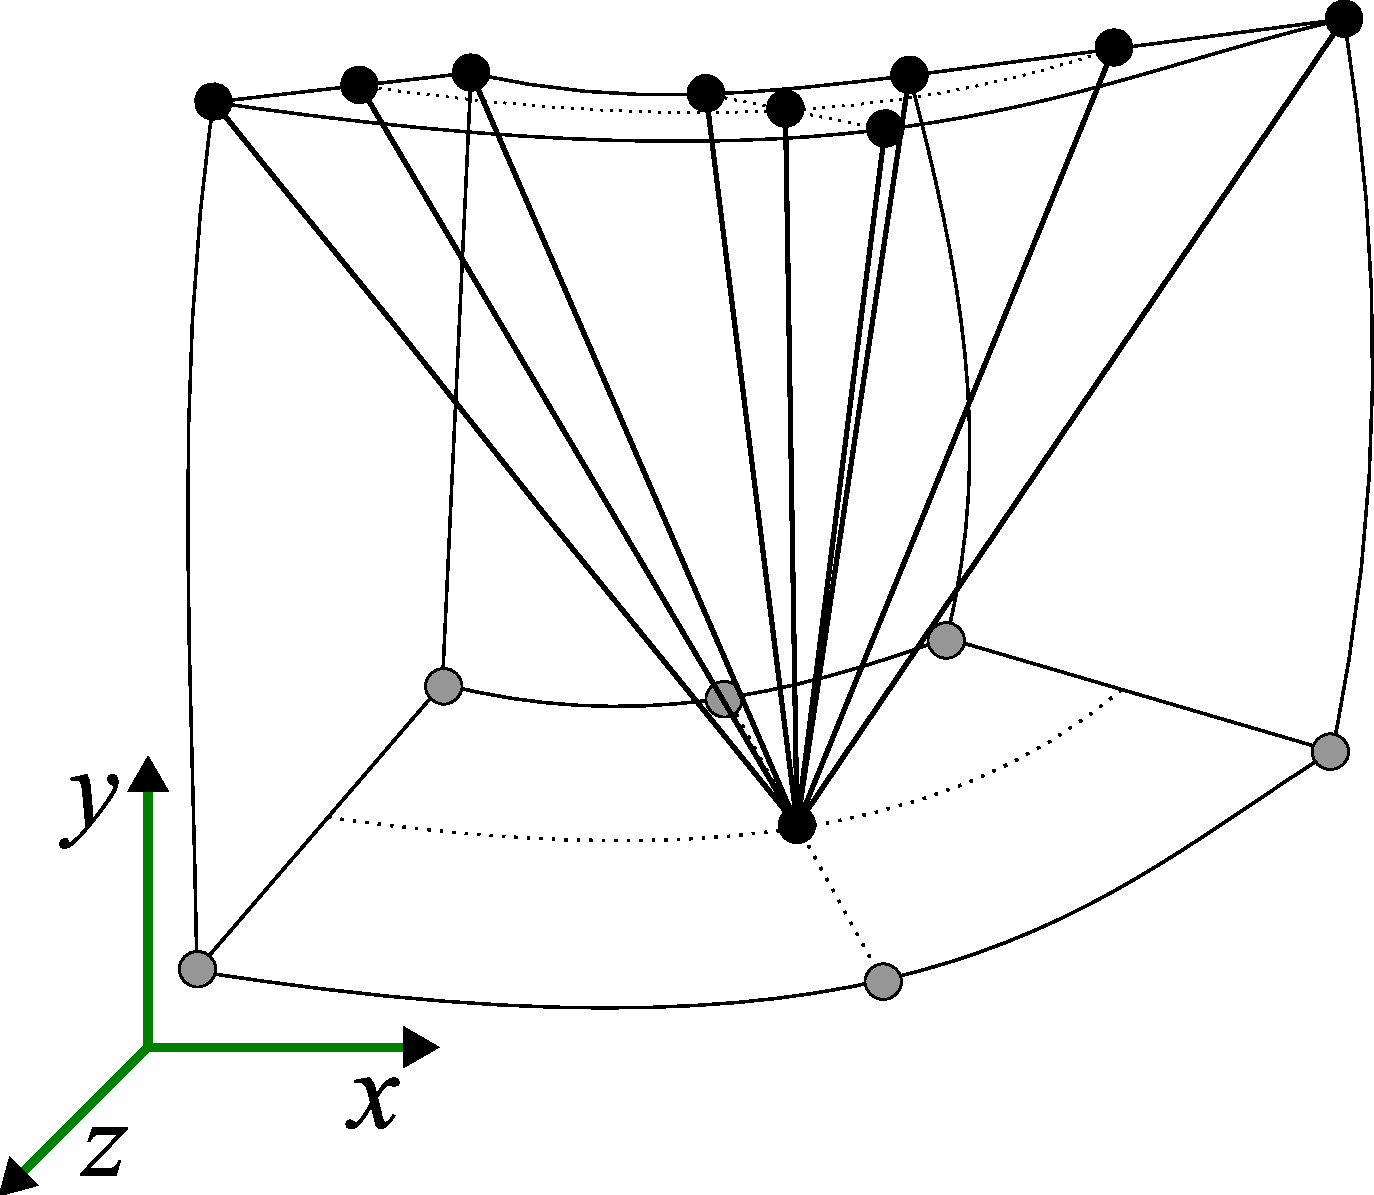
\includegraphics[width=0.35\linewidth, height=0.35\linewidth]{figures/splines_world_space.pdf}}
    \subfigure[$\xi$ space]{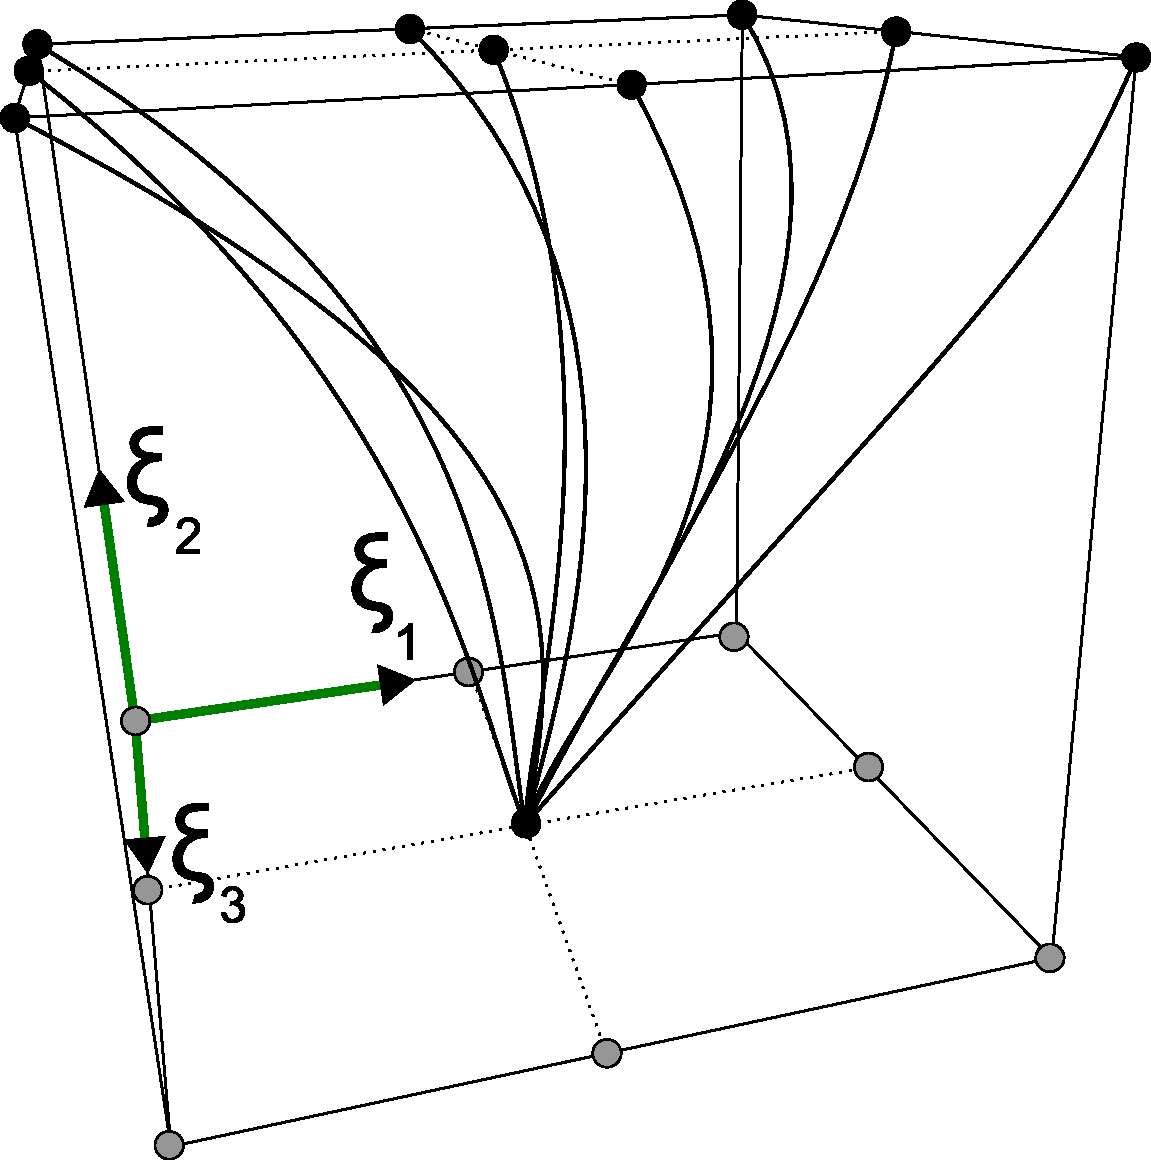
\includegraphics[width=0.35\linewidth, height=0.35\linewidth]{figures/splines_xi_space.pdf}}
    \subfigure[world $\mapsto \xi$]{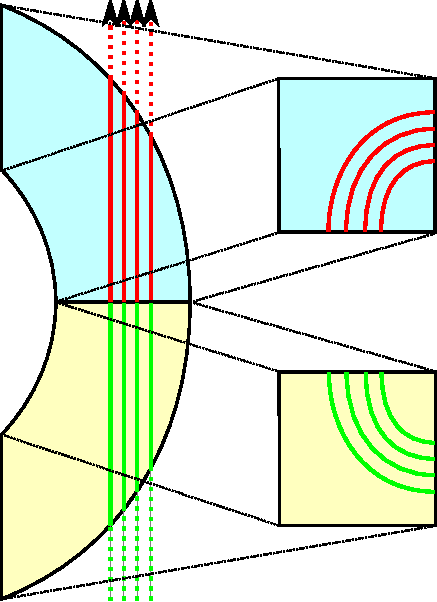
\includegraphics[height=0.35\linewidth]{figures/viewingrays.pdf}}
    \caption{Transforming straight rays given in world space, {\it (a)}, to $\xi$ space, {\it (b)}, causes these rays to be curved. View rays that are parallel and similar in world space, {\it (c,left)}, will be projected to similar curves in $\xi$ space, {\it(c,right)}. The dots show the points used for calculating the proxy rays shown, with the dotted lines emphasizing the relevant face.}
    \label{fig:raycoords}
\end{figure}

When visualizing such models world coordinates are usually more convenient to use, as they define the position and orientation of the elements. As soon as the dependent variables have to be accessed however, the $\xi$ coordinates need also be taken into account as the dependent variables can only be accessed through transformation into $\xi$ space. Thus, the world coordinate system can be used for finding ray intersection points with the elements, while the actual ray traversal is performed in $\xi$ space. As can be seen in Figure~\ref{fig:raycoords}, this transformation affects the geometry of the viewing rays, which can end up as curves in $\xi$ space. While the transformation from $\xi$ space to world space can be computed fairly easy as $x(\xi)=\sum_{i=1}^n x_i \phi_i(\xi)$, for $n$ nodal coordinates, $x_i$, and basis functions, $\phi_i$, the inverse transformation required during ray-casting is computationally much more demanding. Numerical methods, for example the multi-dimensional Newton method~\cite{Press92}, which are often applied to perform this transformation, involve high computational complexity and thus are not feasible in an interactive context. Therefore alternative approaches are necessary to avoid the computational complexity of the world to $\xi$ space transformation in the rendering stage of the visualization pipeline.
%
%
%
\section{Coherency-based Curve Compression}\label{sec:preprocessing}
In this section we present the basis for a novel ray-casting based algorithm for the interactive exploration of curvilinear FE models.

The \emph{straightforward approach} for ray-casting FE models would be to march along a ray in world space and transform each world space sample coordinate, $x$, into its corresponding material coordinate, $\xi$, before accessing the dependent variables. As shown in Table~\ref{tab:performance}, this approach is computationally very demanding and therefore cannot, in general, be performed at interactive frame rates. By using our approach we are able to shift this, originally view-dependent, computation from the rendering stage into the data processing stage of the visualization pipeline. Thus, we can reduce the computational load during rendering and achieve interactive frame rates when volume rendering curvilinear FE models.

To perform the desired shift from the rendering stage into the data processing stage, we exploit the following key observations about the degree of coherency of curvilinear FE models. FE method grids are designed to minimize approximation errors in the solution and to ensure convergence. In particular the Jacobian of the world-to-material coordinate mapping must not contain any singularities, and the grid resolution needs to be high enough that variations of the unknown variables can be approximated adequately with the underlying FE basis functions~\cite{knupp07meshquality}. This implicit smoothness constraint is exploited in our technique since it also limits the shape variations of neighboring rays in world coordinates mapped into $\xi$ space, i.\,e., we can assume some degree of intra-element coherency between adjacent rays. Because the Jacobian does not contain singularities we can employ the Newton method, or similar solvers, to compute the inverse of the world-to-material coordinate mapping.

Many FE applications also require some degree of inter-element compatibility, and some degree of symmetry and self-similarity. These characteristics result in a FE mesh with clusters of similar elements, and hence some degree of inter-element coherency. Figure~\ref{fig:raycoords}~(c) illustrates this coherency as it shows the shape of rays in $\xi$ space ({\it right}), which adjacently traverse world space ({\it left}).

In addition, coherency is supported as most models in practical applications need well-behaved elements, i.e.\,low distortion and an aspect ratio close to one, in order to result in a stable numerical simulation. The approach presented uses precomputation, which is performed within two preprocessing steps as shown in Figure~\ref{fig:workflow}. In the first step, we compute a high number of proxy rays in $\xi$ space. These proxy rays act as a view- and resolution-independent spline representations of the actual viewing rays that are cast through the $\xi$ space during rendering. In the second step, we exploit inter- and intra-element coherency to reduce the vast number of proxy rays to a representative subset, which is then used during GPU-based ray-casting in the third step. By exploiting the precomputed data FE models can be explored interactively by changing the transfer function and other rendering parameters. The following two subsections describe the two preprocessing steps, while the GPU-based ray-casting is discussed in Section~\ref{sec:rendering}.
%
\begin{figure}[b]
	\centering
	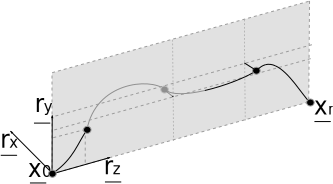
\includegraphics[width=0.75\linewidth]{figures/splinetransformation_new}
	\caption{To achieve a higher degree of similarity during the curve clustering we exploit the orientation invariance of the proxy rays and transform them into a common coordinate system where the principal curve axis coincides with the $z$-axis. Furthermore we exploit scale invariance to align all exit points.}
	\label{fig:proxyrayalignment}
\end{figure}
%
%
%
\subsection{Proxy Ray Generation}\label{subsec:proxyraygeneration}
To be able to compute a complete set, $R$, of proxy rays, it is essential that it covers all parts of the FE model. This means that both the world and the $\xi$ space are densely populated with straight and curved rays, respectively. However, since the view direction used during rendering affects the ray traversal direction and the proxy rays are directional, it is not sufficient that all positions within an element are close to a single proxy ray; they must also be close to proxy rays having different directions. As the interpolation functions in $\xi$ space can, in principle, be different for each element within one FE model, elements are treated individually during preprocessing and rendering. Finding the desired dense and omnidirectional proxy ray population for an element can be performed in two ways. It can either be done adaptively, by analyzing the actual ray distribution within each element to find areas of high importance and create more rays for these areas, or in a uniform way over each element. As our algorithm is based on the inter- and intra-element coherency the latter distribution is sufficient since we assume a continuity between neighboring rays without high frequency changes.

To obtain such a proxy ray distribution we exploit the intra-element coherency, which is the result of a high similarity between rays in $\xi$ space that enter and exit an element through adjacent coordinates. Therefore we compute a dense and uniform distribution, $P$, of potential entry and exit points on the surface of each element. While these points should be distributed over the entire surface of an element, the requirements with respect to the uniformity of $P$ are rather loose due to the intra-element coherency. We distribute the potential entry and exit points by performing an equidistant subdivision of all faces of an element. In this step the subdivision parameter, $s_f$, controls the number of points equidistantly positioned along the $u$ and the $v$ coordinates of a face. Thus the density of $P$ can be directly controlled by changing the subdivision parameter, $s_f$. To reduce the number of initially generated proxy rays it would also be an option to vary $s_f$ based on the extents of a face in world space. In cases where an element is strongly deformed however, such that one face is much smaller than other faces, this usually indicates strong variations in the FE simulation which makes a higher sample density in world space necessary. Therefore we have decided to choose a constant, but sufficiently high, $s_f$ for the proxy ray generation.

The actual proxy rays are then computed based on the resulting point distribution, $P$. To obtain proxy rays from $P$ we consider all pairwise combinations $(p',p'')$, with $p',p'' \in P$. During rendering a ray intersecting $p'$ and $p''$ would be a line in world space and a curve in $\xi$ space. Figure~\ref{fig:raycoords} shows an example of 9 rays going from one point of a face to all points of the opposite face. When connecting $p'$ and $p''$ with a straight line, representing a viewing ray in world space, the proxy ray in $\xi$ space can be obtained by sampling along the straight line and transforming each sample's position into $\xi$ space. While this sampling is performed with a fixed but sufficiently high sampling rate $s_r$, it should be pointed out that it does not represent or determine the sampling rate used later during rendering. $s_r$ is only used to obtain the geometry of the proxy rays, whereas the sampling rate used for the compositing during ray-traversal in the rendering step can still be chosen independently.

As the set of proxy rays, $R$, has to be dense its size is obviously a limiting factor. Assuming that our subdivision parameter, $s_f$, would result in $n$ points along the $u$ and the $v$ coordinate of an element's face, we would have $n^2$ grid points on each face. Thus we would have $n^2\cdot\left|F\right|$ grid points in total, assuming that each element has $\left|F\right|$ faces. This would result in $r_t = (n^2 \left|F\right|)^2$ proxy rays to be precomputed. Though we have kept $s_f$ constant to allow a less complex implementation of the ray-casting process, we have other possibilities to reduce the size of $R$. To achieve this reduction we exploit properties of the standard volume rendering integral which is used in the rendering stage:

$$ L(x,\omega_o) = L_0 \cdot e^{-\int_{x_0}^{x}\kappa(x'')dx''} + \int_{x_0}^{x}  \! c(x') \cdot e^{-\int_{x'}^{x}\kappa(x'')dx''} dx'$$

\noindent where $c(x')$ represents the emissive color at sample $x'$ and $e^{-\int_{x_0}^{x}\kappa(x'')dx''}$ represents the exponential falloff between $x_0$ and $x$. When exploiting this rendering integral the same observations hold as when applying the integral within the context of regular volume rendering. For a ray cast through a medium the application of this integral results in an exponential falloff, i.\,e., when the ray is cast from one start point, $x_0$, to one end point, $x_n$, the samples in the regions surrounding $x_0$ will have considerably more influence on the image than those around $x_n$. In extreme cases where structures with a high degree of opacity are rendered, samples close to $x_n$ do not have any influence at all. To select an optimal proxy ray subset during the precomputation stage we can take this observation into account. Therefore, we can use two different point distribution densities for entry and exit points, which is achieved by replacing $s_f$ with $s_f'$ and $s_f''$. Thus we obtain a point distribution of higher density, representing ray entry points, and a point distribution of lower density, representing exit points. When considering all entry and exit points of these two distributions in a pairwise manner, we achieve an importance-based ray sampling, where rays are more accurately represented when being close to the entry points. In comparison with the $r_t$ rays computed with the uniform proxy ray distribution, the importance-driven ray reconstruction approach results in $r_i = (n_f \cdot \left|F\right|) \cdot (n_b \cdot \left|F\right|)$ rays, where $n_f$ and $n_b$ represent the number of precomputed entry and exit points. This results in a decreased number of proxy rays, where the proxy ray set $R$ is more dense towards the respective entry points and thus better complies with the exponential falloff which occurs during ray-casting. This works best for rather homogeneous parameters, while in cases where all features of interest are located close to the faces a uniform proxy ray distribution is beneficial.

As $s_f$ should be high but independent of the sampling rate used during rendering, it is unfeasible to store the proxy rays based on the precomputed samples. Under the assumption that the proxy rays are well-behaved and at least $C^1$ continuous, we can reduce the memory footprint by storing the proxy rays as parametric curves facilitating a lower number of control points than the original sampling density, $s_f$. We will present the ramifications of different numbers of control points for the error in Section~\ref{sec:results}. Due to the requirements regarding interpolation of the control points, local control, numerical stability, and non-complex evaluation, Catmull-Rom splines~\cite{catmull74splines} are a natural choice for this parametric representation. Furthermore Catmull-Rom splines have built-in $C^{0}$ and $C^{1}$ continuity, thus being continuous in position as well as tangent vector, leading to a smooth curve. Additionally, Catmull-Rom splines allow us to obtain and interpolate the start and end tangent of the curved rays directly.
%
%
%
\subsection{Curve Clustering}\label{subsec:curvecompression}
The curve compression, which is used to obtain a manageable set of proxy rays during rendering, first increases the similarity of the proxy rays by exploiting orientation and scaling invariance, before computing a representative subset using a clustering algorithm, whereby the increased similarity of the proxy rays allows us to compute a smaller subset of proxy rays while maintaining the same quality of compression.

\noindent \textbf{Curve similarity.} In the previous subsection, we have described how to obtain a densely populated set of proxy rays that are represented as parametric curves in $\xi$ space. As this set is too large to be considered during rendering we will eliminate proxy rays from within this set by taking into account the following three observations which increase the similarity. First, a curve does not have a pre-defined entry and exit point order. As the ray traversal and the compositing are performed in the rendering stage we do not need to distinguish between two proxy rays with swapped entry and exit coordinates, if both rays are the same. The second helpful observation refers to the orientation of proxy rays in $\xi$ space. As a proxy ray represents only the traversal path but not the dependent variables accessed during a traversal, we do not need to distinguish between two proxy rays which have the same overall geometry but are differently oriented in $\xi$ space. As long as we know the entry and the exit point of a proxy ray we can orient the proxy ray's geometry such that it is correctly aligned in $\xi$ space. This property is also related to the third observation, the length invariance, which we also exploit to increase the similarity during curve compression. As soon as we know the coordinates of the entry and the exit points we can not only adapt the orientation of a proxy ray but also its scaling. Therefore we do not have to distinguish between proxy rays which have the same geometry but differ only in the scaling factor along their principle axis.

We exploit the three observations stated above in order to achieve a higher degree of similarity during the subsequent clustering-based curve compression. To do so we transform the proxy rays into a common coordinate frame without compromising the uniqueness of each proxy ray as they comply to orientation and scaling invariance. The transformation is done in such a way that the entry point and the exit point lie on the $z$-axis, with the proxy ray's principal axis aligning with the same axis (see Figure~\ref{fig:proxyrayalignment}). To be further able to define the rotation around this axis we take into account the first control point, $c_i$, that is not colinear with the start and end points and transform the proxy ray such that $c_i$ lies in the $yz$-plane. If there is no such point, the proxy ray is a straight line so that it can be rotated to coincide with the z axis. After this transformation, $M_{trans}$, has been applied all proxy rays lie in the same coordinate system as shown in Figure~\ref{fig:proxyrayalignment}, and thus the comparison performed during clustering produces a higher degree of similarity. While this transformation into a common coordinate system indirectly reduces the number of rays, it requires us to store the angle of rotation, $\theta$, for each proxy ray. This is necessary as $\theta$ is required to be able to compute ${M_{trans}}^{-1}$, which is needed during rendering to correctly orient the precomputed proxy rays.

\noindent \textbf{Curve clustering.} To reduce the size of $R$ we exploit the inter- and intra-element coherency discussed above. This allows us to perform clustering in order to obtain a representative subset of $R$, called $R'$. Several algorithms have been proposed for clustering curves and we have decided to exploit the approach proposed by Abraham et al.~\cite{abraham03clustering}. As this approach applies the clustering to the curve coefficients instead of the control points, it can be proven that the derived cluster representatives are optimal candidates. As we have previously increased the curve similarity of the set of proxy rays, $R$, by transforming them into a common coordinate system, we can use a lower number of cluster representatives when using the clustering method. This reduces the data size as well as computation time needed for the clustering. We will show in Section~\ref{sec:results} how the number of clusters affects the achieved quality of the clustering.

Abraham et al. state that the comparison metric used during the clustering is the most crucial part, as it directly defines the similarity of two curves~\cite{abraham03clustering}. Inspired by their work we use the spanned area between two proxy rays as a metric. To compute the spanned area, we equidistantly sample the proxy rays with a high sampling rate, and generate a triangle strip between the sampling points. The similarity can then be expressed by a Riemann sum of the triangle areas. If we have two proxy rays, $a$ and $b$, with their sampled points, $a_1,\dots,a_n$ and $b_1,\dots,b_n$, where due to the transformation $M_{trans}$, $a_1=b_1$ and $a_n=b_n$ holds true, we can calculate the approximate area between the rays. If $x_iy_j$ denotes the vector from $x_i$ to $y_j$, then the similarity of $a$ and $b$ is proportional to:

\begin{eqnarray*}
2\cdot d(x,y) &=& \Vert a_1a_2 \times a_2b_2\Vert + \\
&& \sum_{i=2}^{n-2}\Vert a_ia_{i+1} \times a_ib_i \Vert + \Vert b_ib_{i+1} \times b_{i+1}a_{i+1}\Vert + \\
&& \Vert a_{n-1}a_n \times a_{n-1}b_{n-1}\Vert,
\end{eqnarray*}

It is clear that this function fulfills the metric traits of non-negativity, the identity of indiscernibles and symmetry, since all these properties hold for the area computation as well. Although we could have used the closed solution for the two curves and compute the analytically correct solution, we wanted to use the same metric for non-parametric curves as well. The same metric presented here will be used in the error analysis, where no closed solution for the bent ray is available.

For the actual clustering we exploit the k-means clustering algorithm which was originally presented by Hartigan~\cite{hartigan75kmeans}. It has the benefit that it is robust even with large high-dimensional data, and only needs the number of final clusters and a metric as parameters. Unfortunately the number of clusters is not known a priori and, in fact, there might be no definite answer as to which is the best number in general. To deal with this problem we have evaluated the impact of different numbers of clusters in Section~\ref{sec:results}. Alternatively, one could apply algorithms for finding an optimal number of clusters, such as for instance k-fold cross-validation, which is often used together with k-means. As output, k-means provides the desired number of representative proxy rays, one for each of the clusters. Besides the obtained cluster representatives we need to store for each proxy ray the cluster ID as well as the angle $\theta$ The cluster ID is used to determine the cluster to which it belongs.
%
\begin{figure}[b]
  \centering
      \centering 
      \subfigure{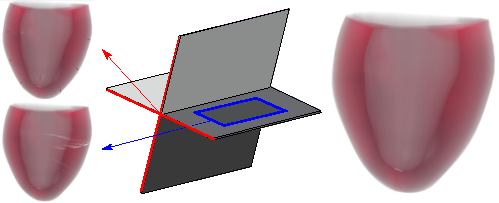
\includegraphics[width=0.30\linewidth, height=0.3\linewidth]{figures/coincidence/Coincidence.pdf}}
      \subfigure{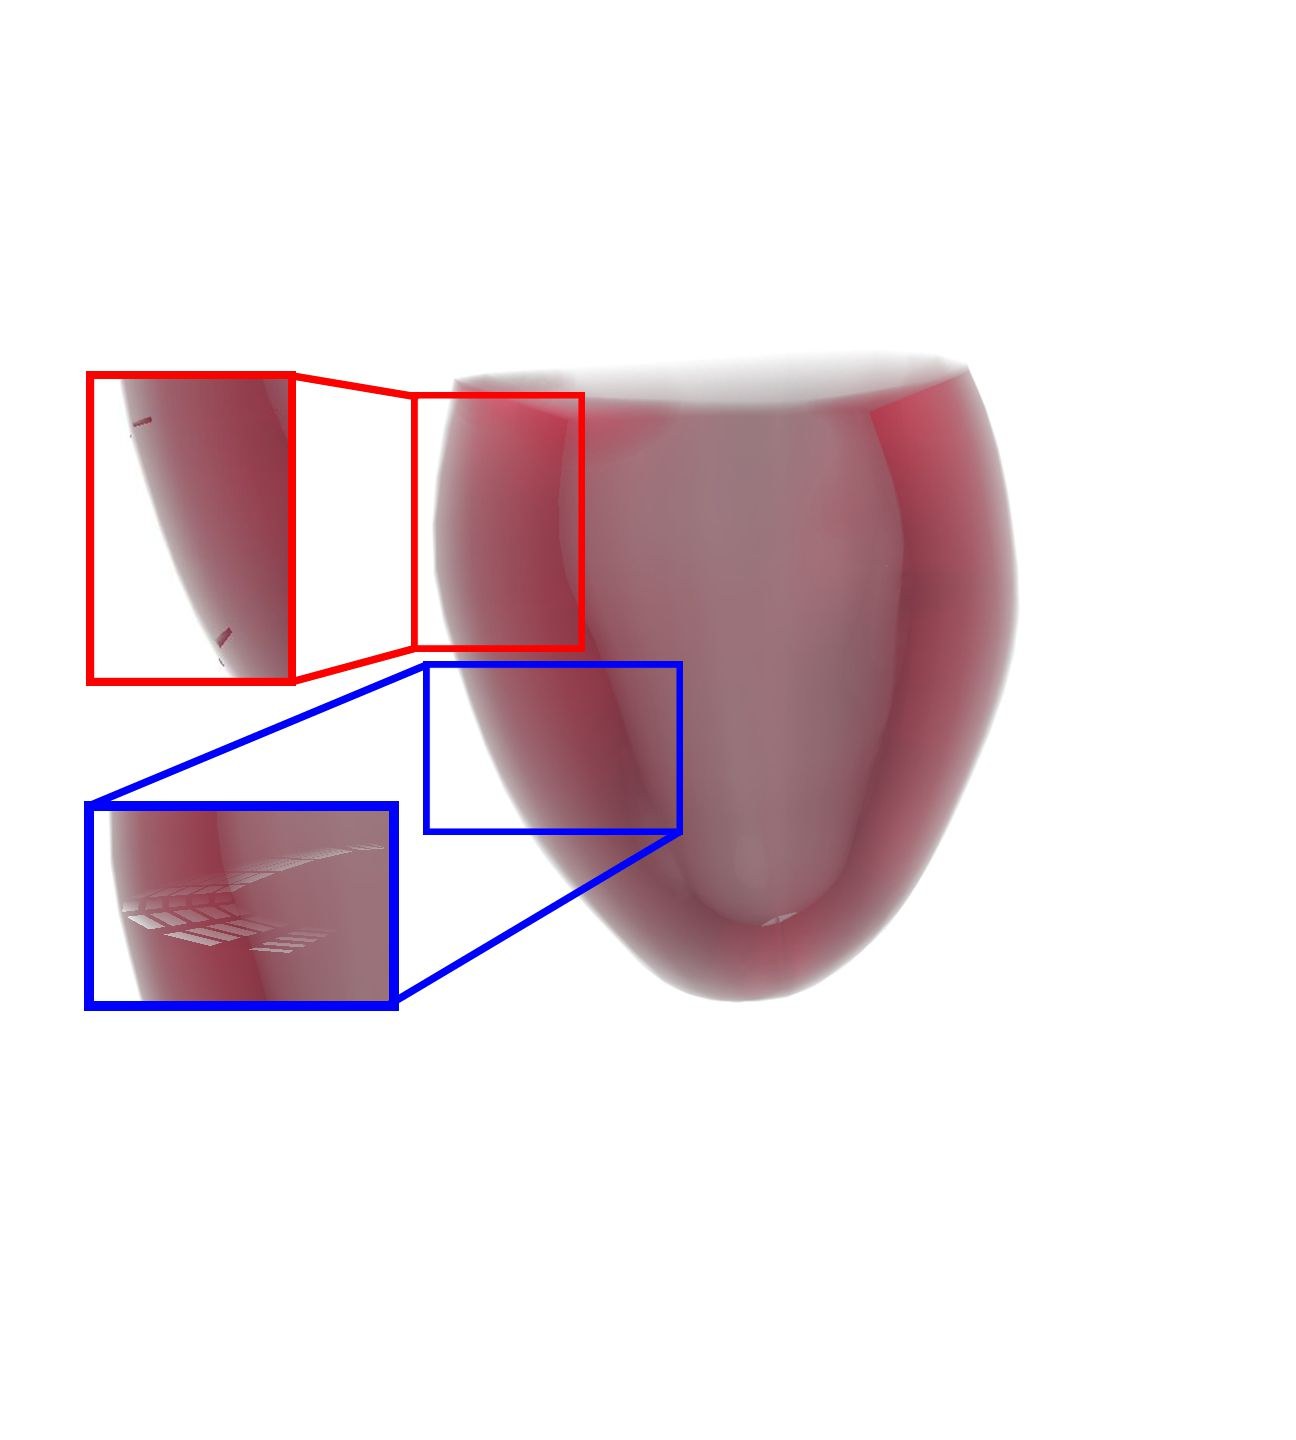
\includegraphics[height=0.3\linewidth]{figures/coincidence/HeartFine_new.jpg}}
  \caption{Two cases of depth coincidence can occur, as illustrated ({\it left}), when rendering adjacent polygons. Point coincidence occurs at the corners of adjacent elements ({\it top}), while surface coincidence occurs at the touching elements' surfaces ({\it bottom}). All coincidences can be avoided ({\it right}).}  
  \label{fig:depthcoincidence}
\end{figure}
%
\begin{figure}[t]
    \centering
    \subfigure[entry world]{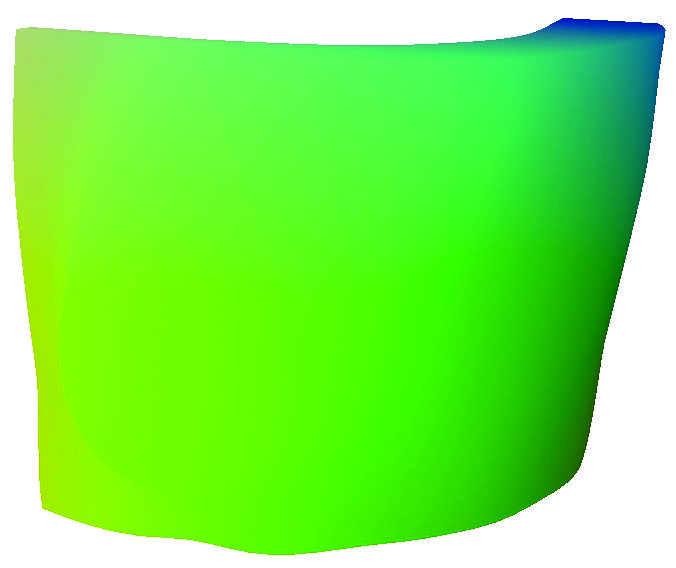
\includegraphics[width=0.18\linewidth]{figures/breast_mesh/BreastEntryWorld1}}
    \subfigure[entry $\xi$]{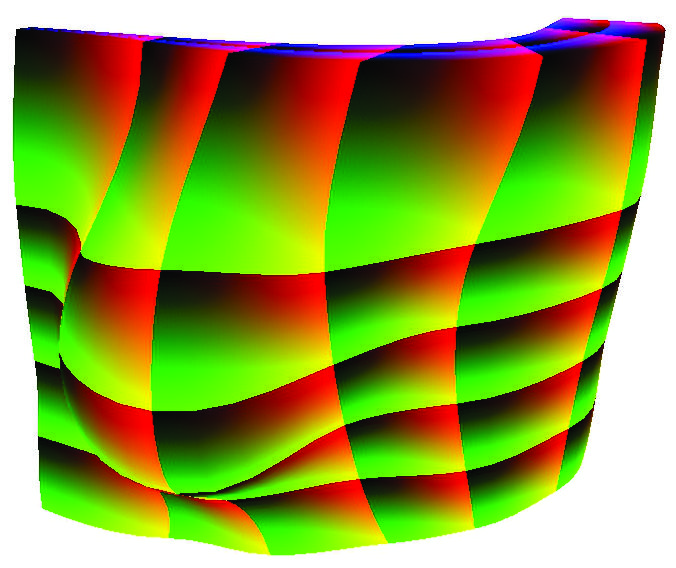
\includegraphics[width=0.18\linewidth]{figures/breast_mesh/BreastEntryXi1} \label{fig:depthpeeling:entryxi}}
    \subfigure[entry depth]{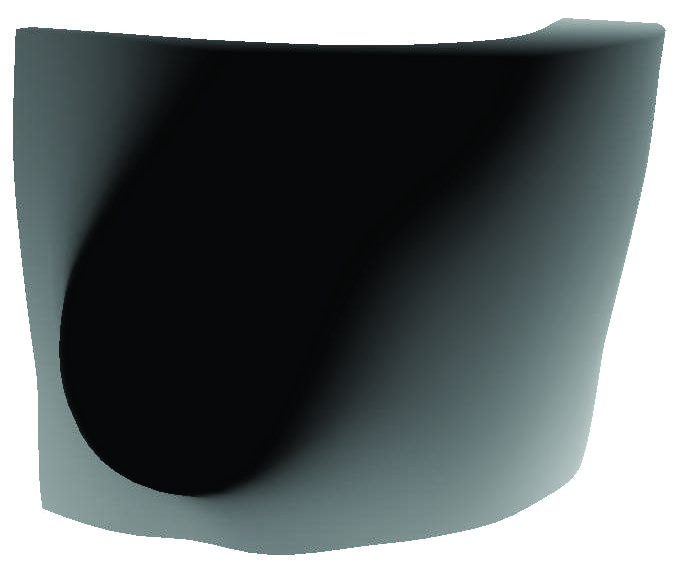
\includegraphics[width=0.18\linewidth]{figures/breast_mesh/BreastEntryDepth1}}
    \subfigure[entry element IDs]{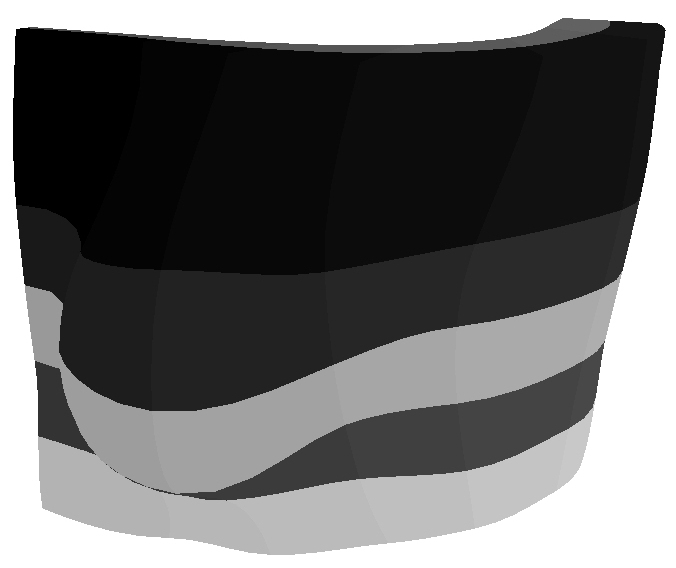
\includegraphics[width=0.18\linewidth]{figures/breast_mesh/BreastElementID1} \label{fig:depthpeeling:entryid}}
    \subfigure[entry face IDs]{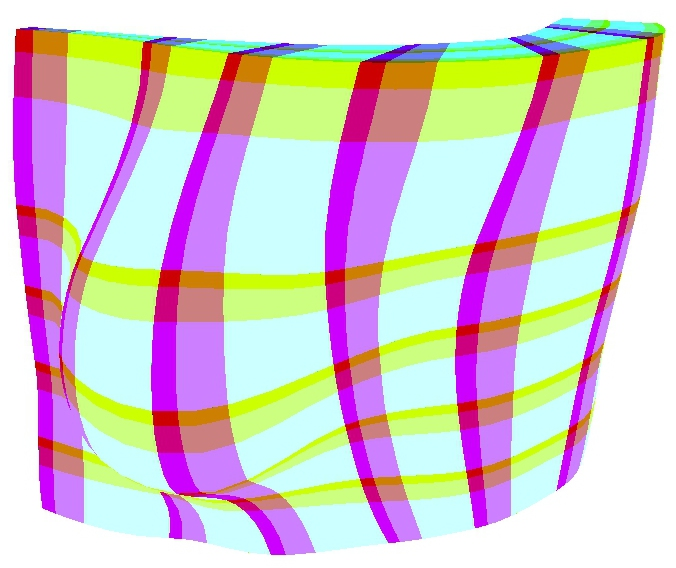
\includegraphics[width=0.18\linewidth]{figures/breast_mesh/BreastEntryFace1}}\\
    \subfigure[exit world]{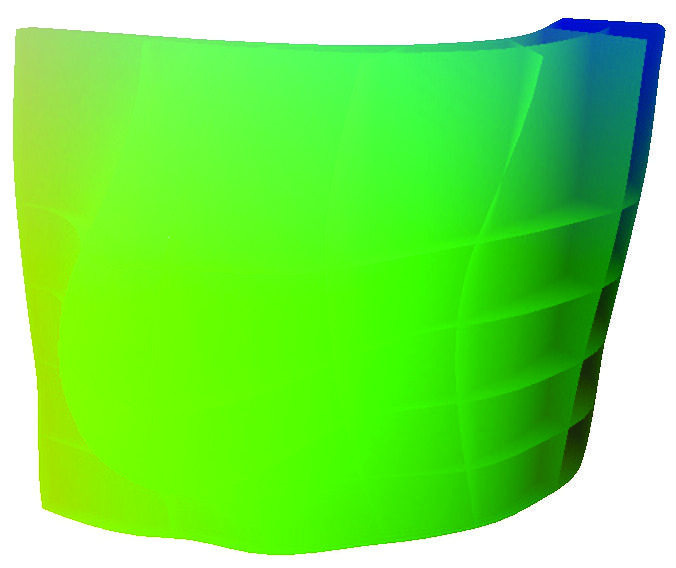
\includegraphics[width=0.18\linewidth]{figures/breast_mesh/BreastExitWorld1}}
    \subfigure[exit $\xi$]{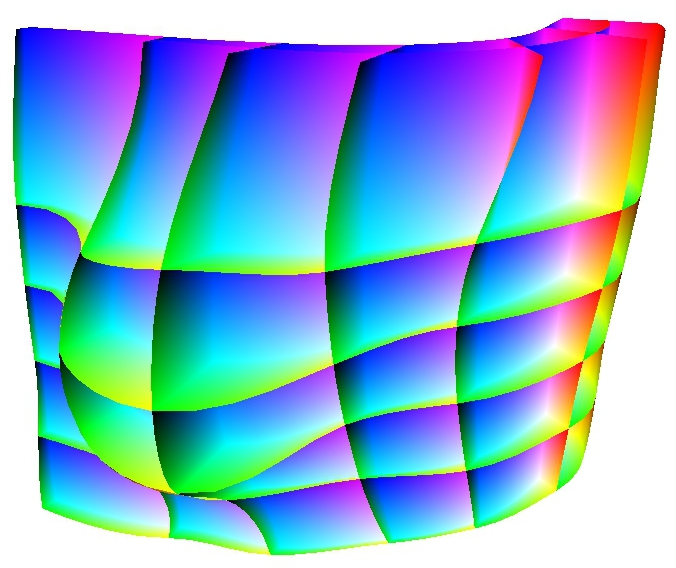
\includegraphics[width=0.18\linewidth]{figures/breast_mesh/BreastExitXi1} \label{fig:depthpeeling:exitxi}}
    \subfigure[exit depth]{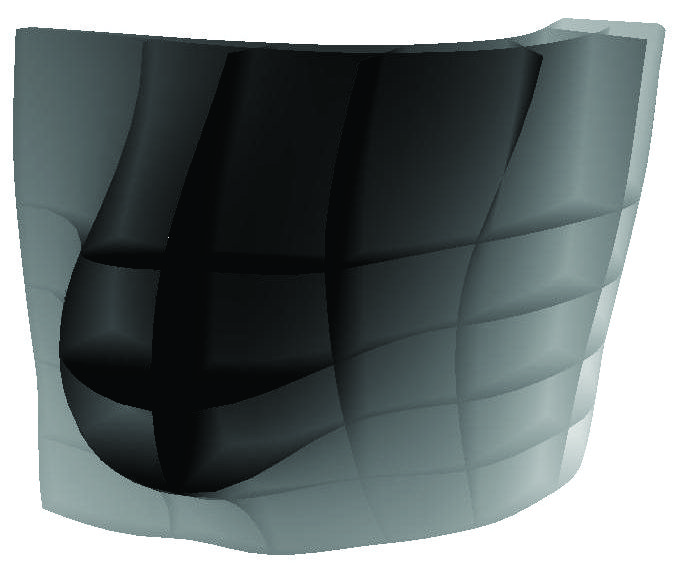
\includegraphics[width=0.18\linewidth]{figures/breast_mesh/BreastExitDepth1}}
    \subfigure[exit element IDs]{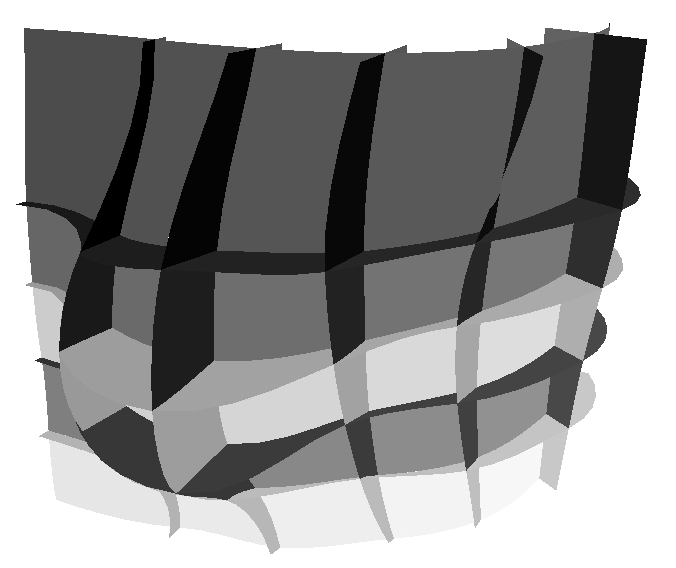
\includegraphics[width=0.18\linewidth]{figures/breast_mesh/BreastElementID2} \label{fig:depthpeeling:exitid}}
    \subfigure[exit face IDs]{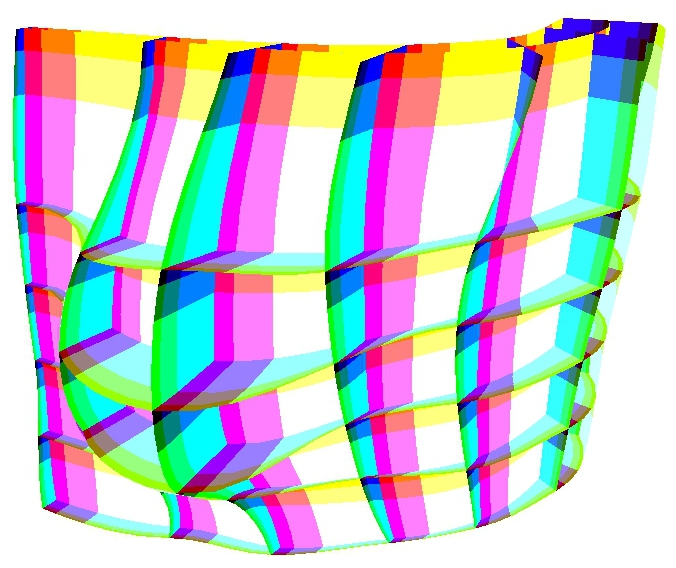
\includegraphics[width=0.18\linewidth]{figures/breast_mesh/BreastExitFace1}}
    \caption{Depth peeling is used to extract the layers of the FE model during rendering. The images show the world coordinates, the $\xi$ coordinate, its depth, the element ID, and the face ID ({\it from left to right}). The first row shows the first depth layer and the second row shows the second depth layer.}
    \label{fig:depthpeeling}
\end{figure}
%
%
%
\section{Bent Ray-Casting}\label{sec:rendering}
While Section~\ref{sec:preprocessing} gives a comprehensive overview of the preprocessing steps needed to obtain the proxy ray set, $R$, and the clustered set, $R'$, the actual rendering process is discussed in detail within this section. We perform GPU-based ray-casting by exploiting the data generated during the preprocessing stage, i.e., all cluster representatives as well as a list, for each proxy ray, storing the associated cluster ID and the rotation angle $\theta$. As the elements are treated individually we need a way to be able to associate ray segments with the elements. Thus the rendering stage is divided into three substages. First element peeling which allows us to obtain the entry and exit points for each element. Second ray marching, where a ray in $\xi$ space is reconstructed from the preprocessed data before it is traversed. Third ray interpolation, which is used to be able to deal with less dense proxy ray sets $R$. These three substages are discussed in the following three subsections.
%
%
%
\subsection{Element Peeling}\label{subsec:peeling}
As the FE models consist of several elements they will, in general, overlap in image space. Therefore mechanisms are needed to determine which sequence of proxy rays best represents a specific pixel. To obtain this sequence of proxy rays we employ a modified depth peeling approach~\cite{mammen89DepthPeeling}. With this approach we can peel away, layer-by-layer, from the rendered FE model by using an additional depth comparison. When using depth peeling however, it is crucial to be able to distinguish between different fragments solely based on their depth values. Unfortunately, in our case this is not possible. As a FE model consists of several adjacent and touching elements, coinciding depth values are common and need to be handled robustly. As illustrated in Figure~\ref{fig:depthcoincidence}, two cases of depth coincidence occur. Point coincidences occur at the corners of adjacent elements~({\it top}) and surface coincidences occur where two adjacent elements' surfaces are touching~({\it bottom}). To deal with this issue we have implemented multi-layer depth peeling, where we take advantage of several attributes to resolve the depth coincidences without introducing errors. Figure~\ref{fig:depthpeeling} shows the employed information next to the color coded $\xi$ and world space coordinates of the first two layers of a FE model. Besides the depth values we also take into account the current element's ID, as well as the ID of the current face in our peeling approach. Thus we can resolve the described coincidence cases and retrieve the entry and exit points for the current view ray segment. This allows us to fetch the cluster representative for this pair (see Section~\ref{sec:implementation}) and perform the ray marching.
%
%
%
\subsection{Ray Marching}
\begin{figure}[t]
    \centering
    \subfigure[Precomputed proxy rays with $s_f$ = 2]{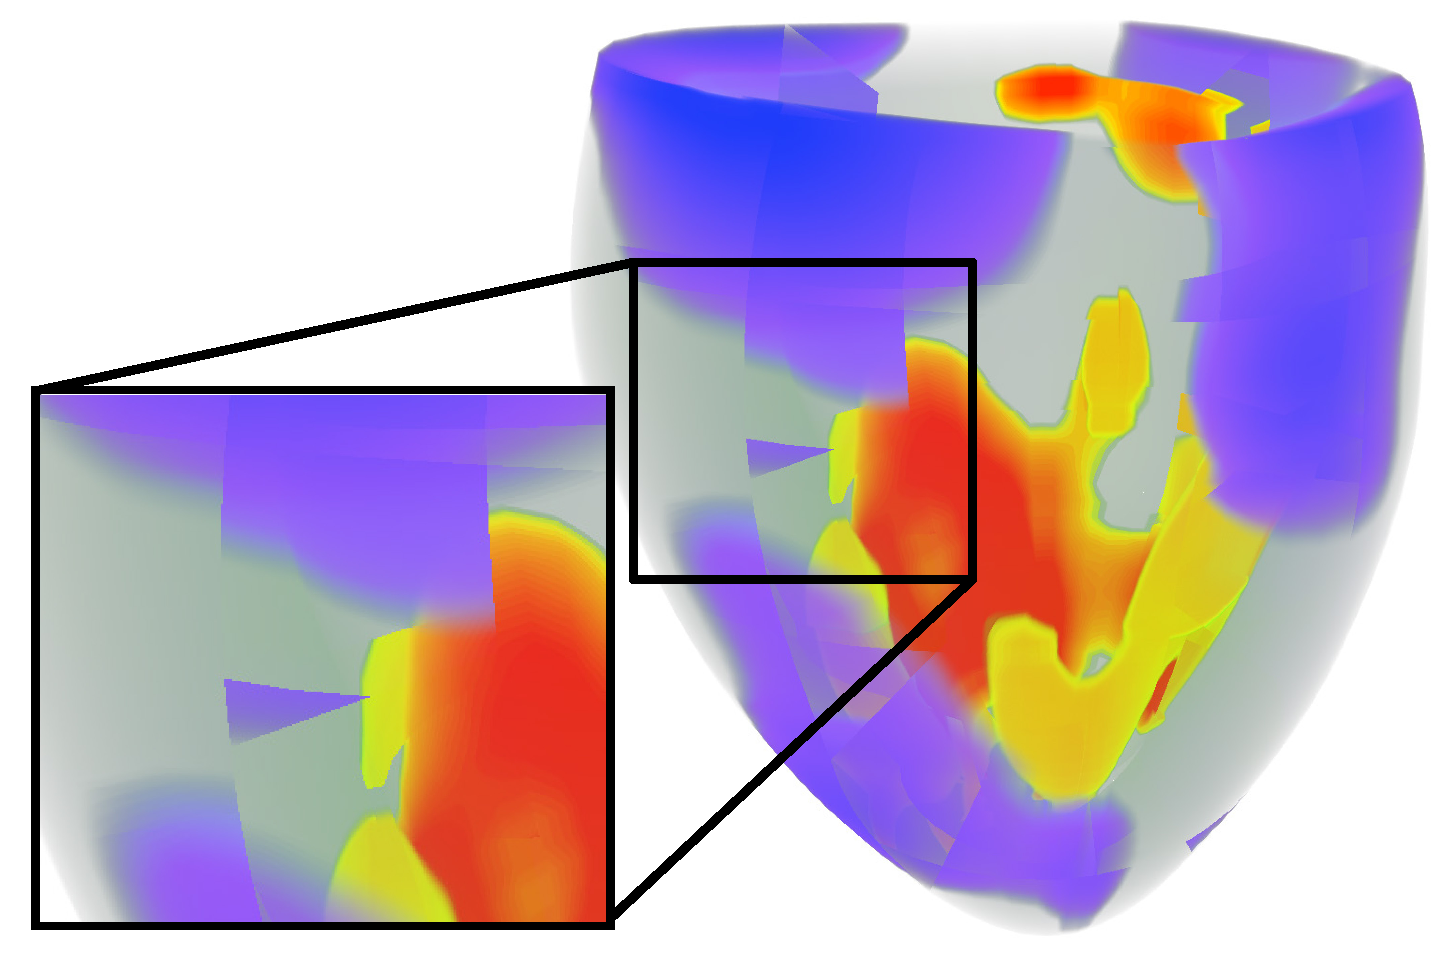
\includegraphics[width=0.39\linewidth]{figures/heart-2-new-with-closeup.pdf}
    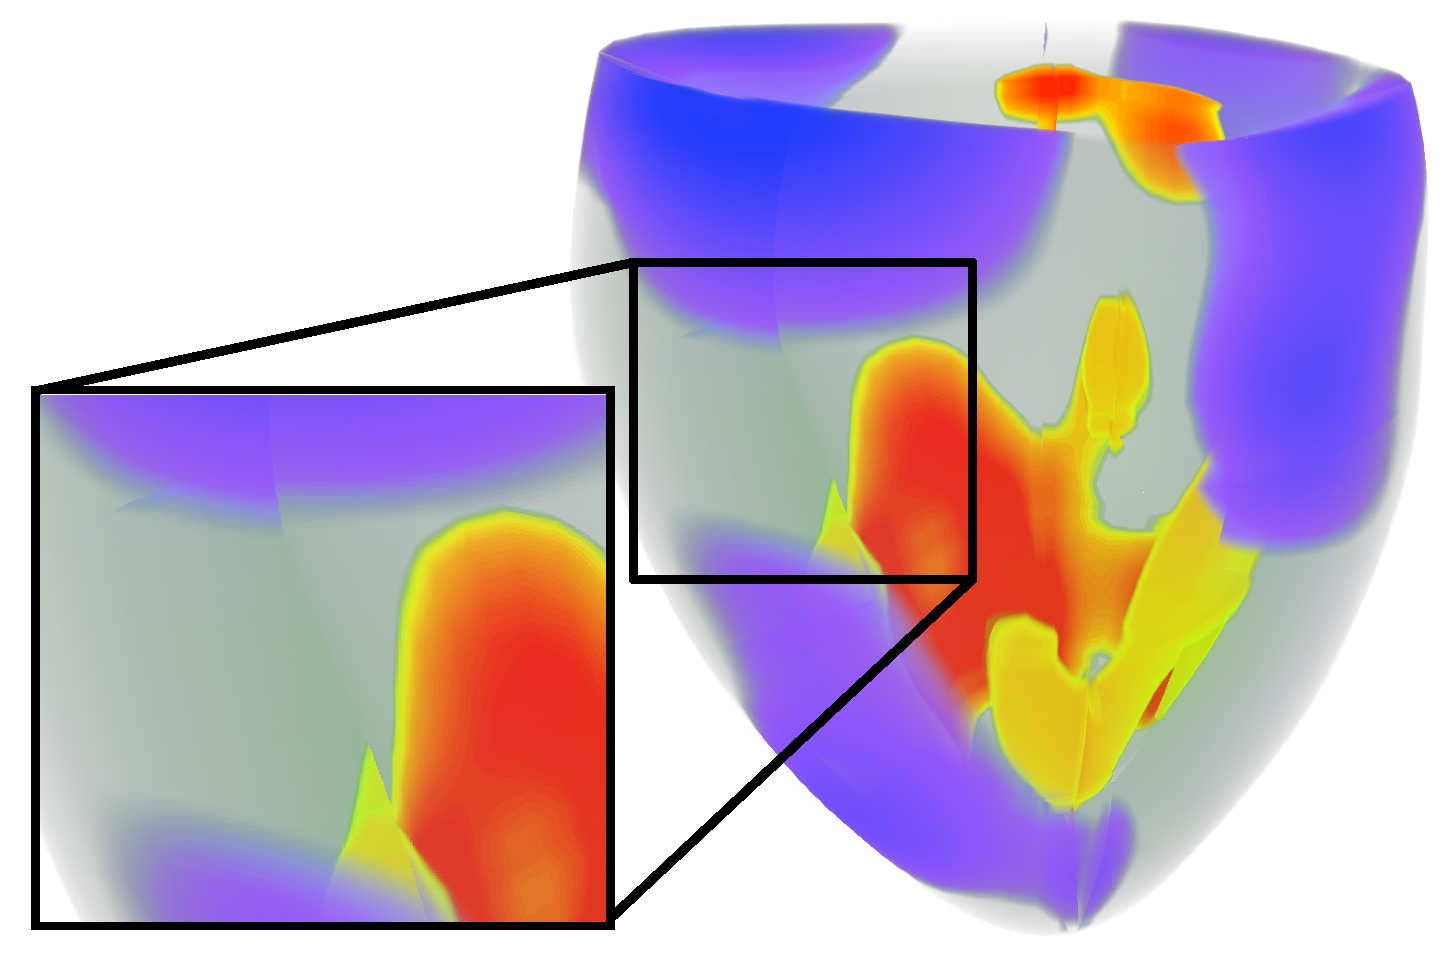
\includegraphics[width=0.39\linewidth]{figures/heart-2-rr-ii-new-with-closeup.pdf}}\\
    \subfigure[Precomputed proxy rays with $s_f$ = 10]{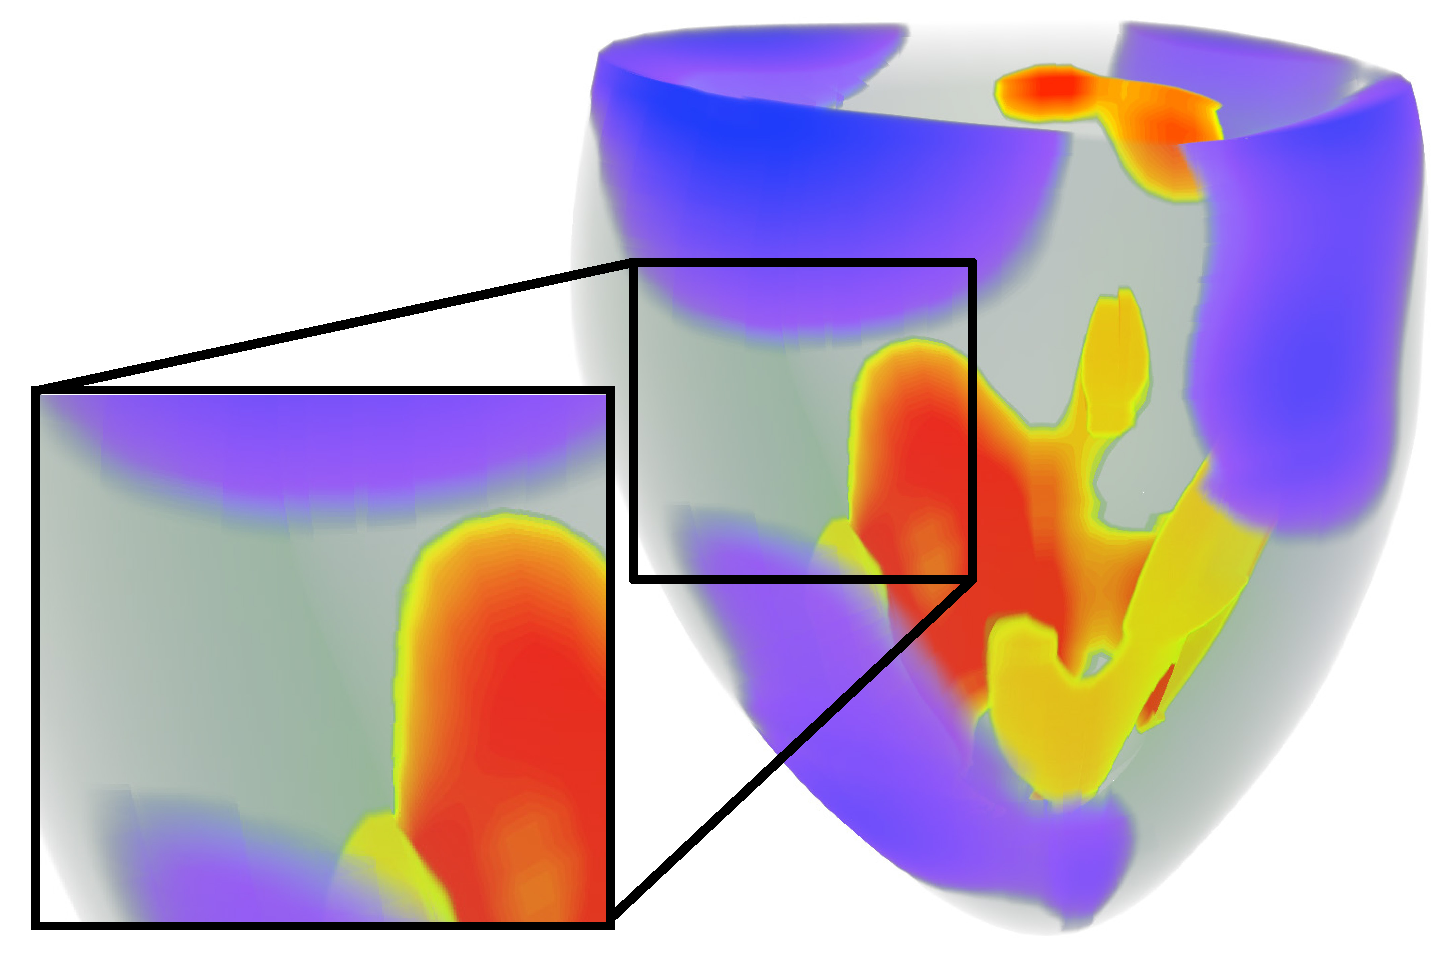
\includegraphics[width=0.39\linewidth]{figures/heart-10-new-with-closeup.pdf}
    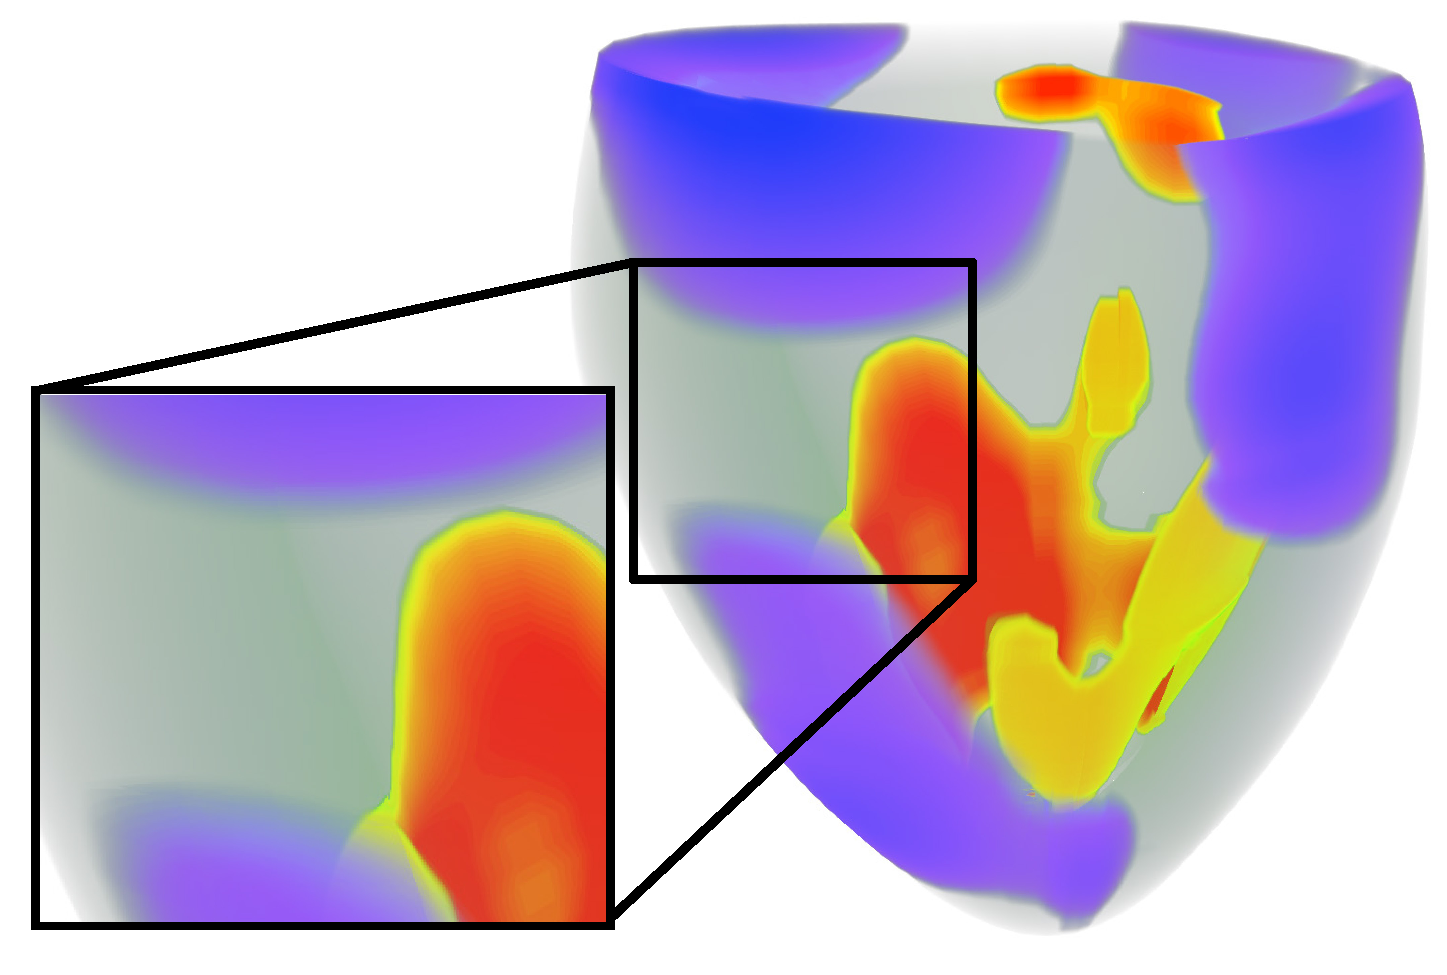
\includegraphics[width=0.39\linewidth]{figures/heart-10-rr-ii-new-with-closeup.pdf}}
    \caption{Results of our approach with two different parameter sets. The first row shows a precomputation with a grid parameter of $s_f$ = 2 and the second with $s_f$ = 10. Within each row we show the application of standard ray interpolation ({\it left}) as well as intra- and inter-ray interpolation ({\it right}). As shown in the close-ups, intra- and inter-ray interpolation reduces noticeable artifacts. Artifacts are still noticeable with $2 \times 2$ proxy rays, as shown in ({a, \it right})}
    \label{fig:rayinterpolation}
\end{figure}

Once we know which proxy ray information needs to be accessed, we can reconstruct its ray geometry by retrieving the spline coefficients for the obtained cluster ID. The reconstructed spline is then transformed back from the canonical orientation along the $z$-axis by applying ${M_{trans}}^{-1}$, such that the spline lies between the entry- and the exit-point of the actual viewing ray in world coordinates. Although the reconstructed spline is similar for pixels in a local neighborhood, the specific path is different because it is fitted to the specific entry and exit-point combination of the viewing ray. Once the proxy ray has been transformed back into its original location we can march along it and perform the actual bent ray-casting by fetching the dependent variables from the $\xi$ space using our spline representation. The expensive world-to-material transformation that would be necessary in the straightforward approach is replaced by an evaluation of the precomputed spline representation. 
%
\begin{figure}[b]
    \centering
    \subfigure[Equidistant sampling]{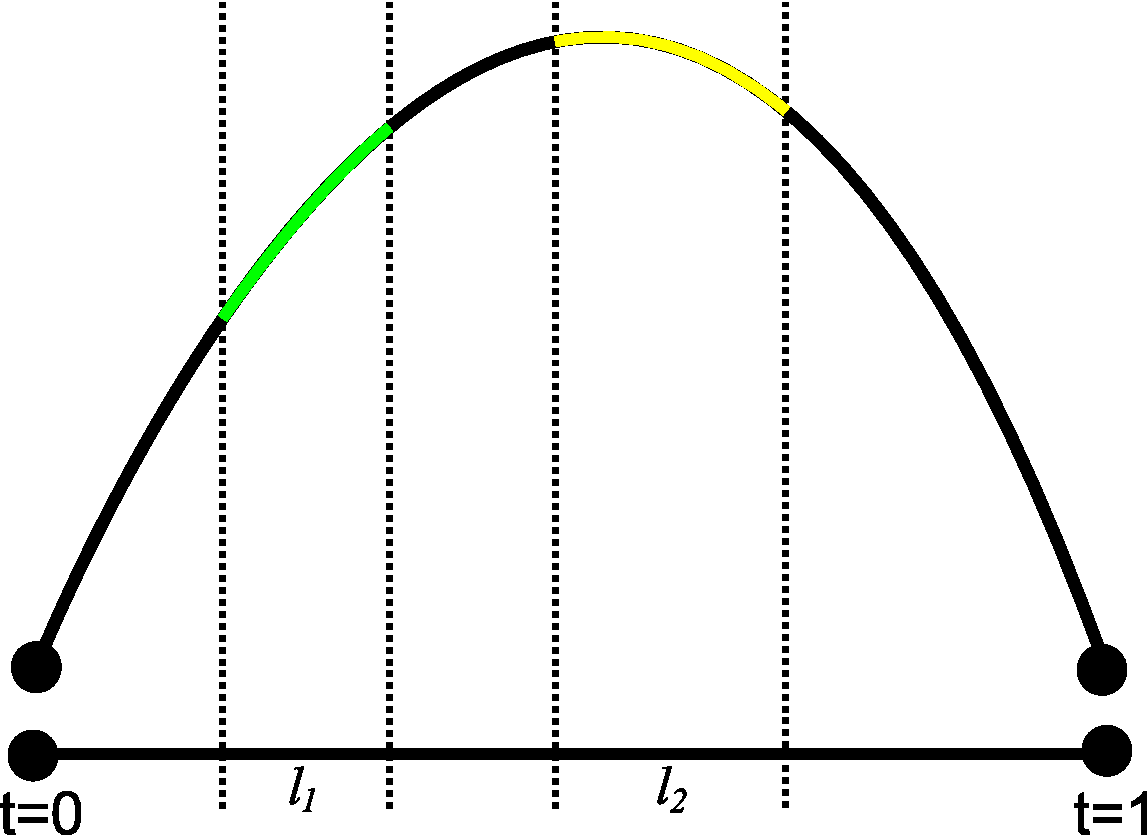
\includegraphics[width=0.32\linewidth, height=0.32\linewidth]{figures/arclength.pdf}\label{fig:arclength}}
    \hspace*{1cm}
    \subfigure[Boundary handling]{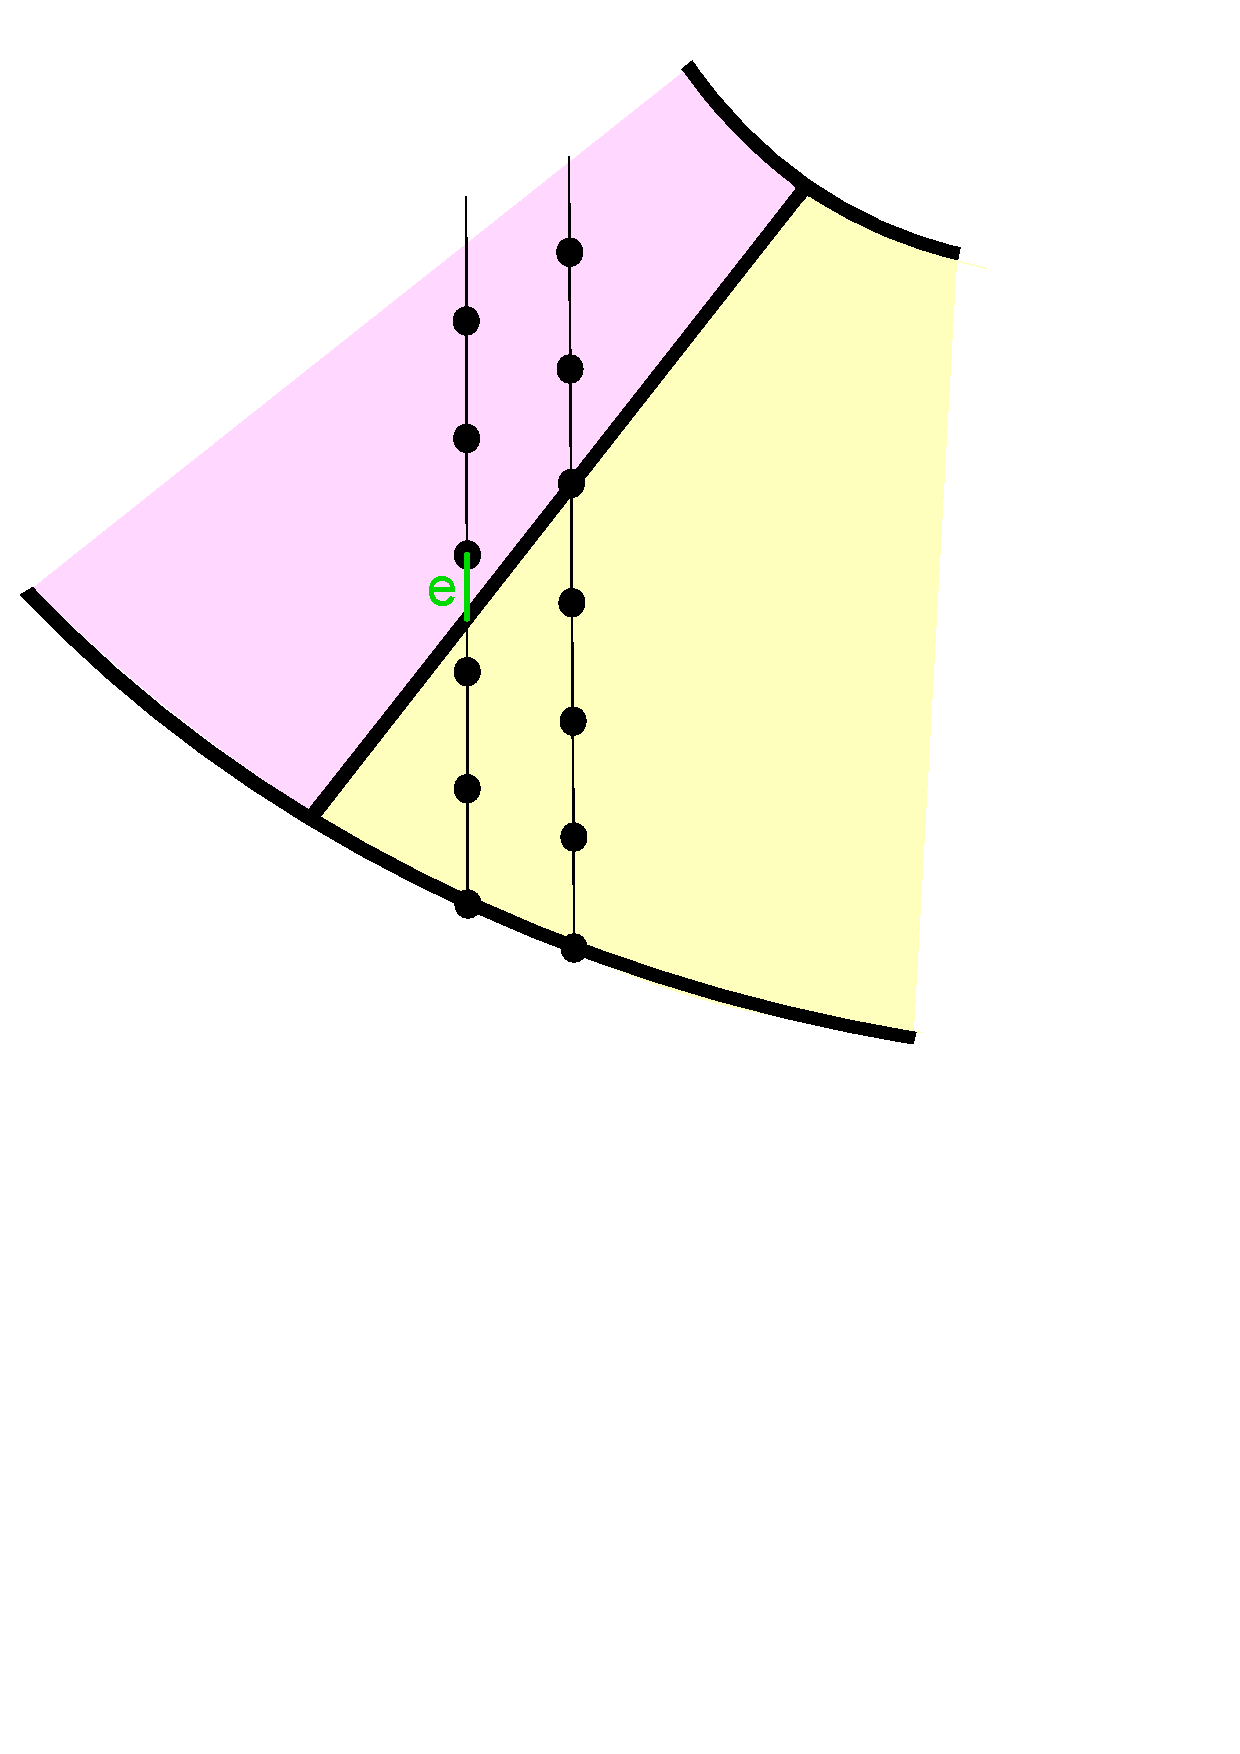
\includegraphics[width=0.32\linewidth, height=0.32\linewidth]{figures/overshoot.pdf} \label{fig:overshoot}}
    \caption{\subref{fig:arclength} To achieve equidistant sampling along a ray in $\xi$ space ({\it top}), an arc length parametrization is applied resulting in a non-uniform sampling in world space ({\it bottom}). \subref{fig:overshoot} Rays penetrating multiple elements must be processed such that constant sampling step sizes are obtained at the borders. The overshoot, $e$, of the first element can be used to offset the first sampling point in the next element.}
    \label{fig:arclengthandovershoot}
\end{figure}

To ensure that we consider possible high-frequencies in the material data, we need to ensure an equidistant sampling along the reconstructed ray in material space in order to obtain optimal results. The proxy rays, however, are parameterized by the parameter value $t \in [0,1]$ in world coordinates which does not take the shape of the ray in $\xi$ space into account, i.e., given a spline $s$, $\Vert s(x) - s(y) \Vert \neq \Vert x - y \Vert$. That means that an equidistant sampling in world space will result in sampling points that are not equidistant along the curve in $\xi$ space. As illustrated in Figure~\ref{fig:arclength}, we address this problem by using an arc length parametrization as presented by Guenter and Parent~\cite{guenter90arclength}. This leads to a function $t \mapsto t'$. If the sampling is done using $t'$ instead of $t$, the sampled values will be equidistant along the curve in $\xi$ space. To ensure accuracy w.r.t. the rendering integral, we employ the equidistant spacing in $\xi$ space to access the dependent variables, but use the distance in world space for the opacity computation.

The subdivision of a curve ray penetrating the whole FE model into segments, based on the penetrated FEs, requires an appropriate border handling scheme. If we sample the ray equidistantly, in a na\"ive way, the last point on the ray, which lies on the exit face of a FE, will, in general, not coincide with an intended sampling point. Special consideration is needed when handling a ray, $a$, that is divided into two segments, $r$ and $s$, in such a way that $r_n = s_0$, i.\,e., the last sample point of $r$ is the first sample point of $s$. In this situation we would have an equidistant sampling rate of $\left|a_i - a_{i+1}\right| = \delta$ for the two rays. However, the na\"ive implementation will result in $\left|r_{n-1} - r_{n}\right| \neq \delta$. To remedy this, we do not sample the last point on each ray but save the distance $\left|r_{n-1} - r_{n}\right|$ instead and use it as an offset for the first sampling point in the next ray segment (see Figure~\ref{fig:overshoot}).
%
%
%
\begin{figure*}[t]
    \centering
    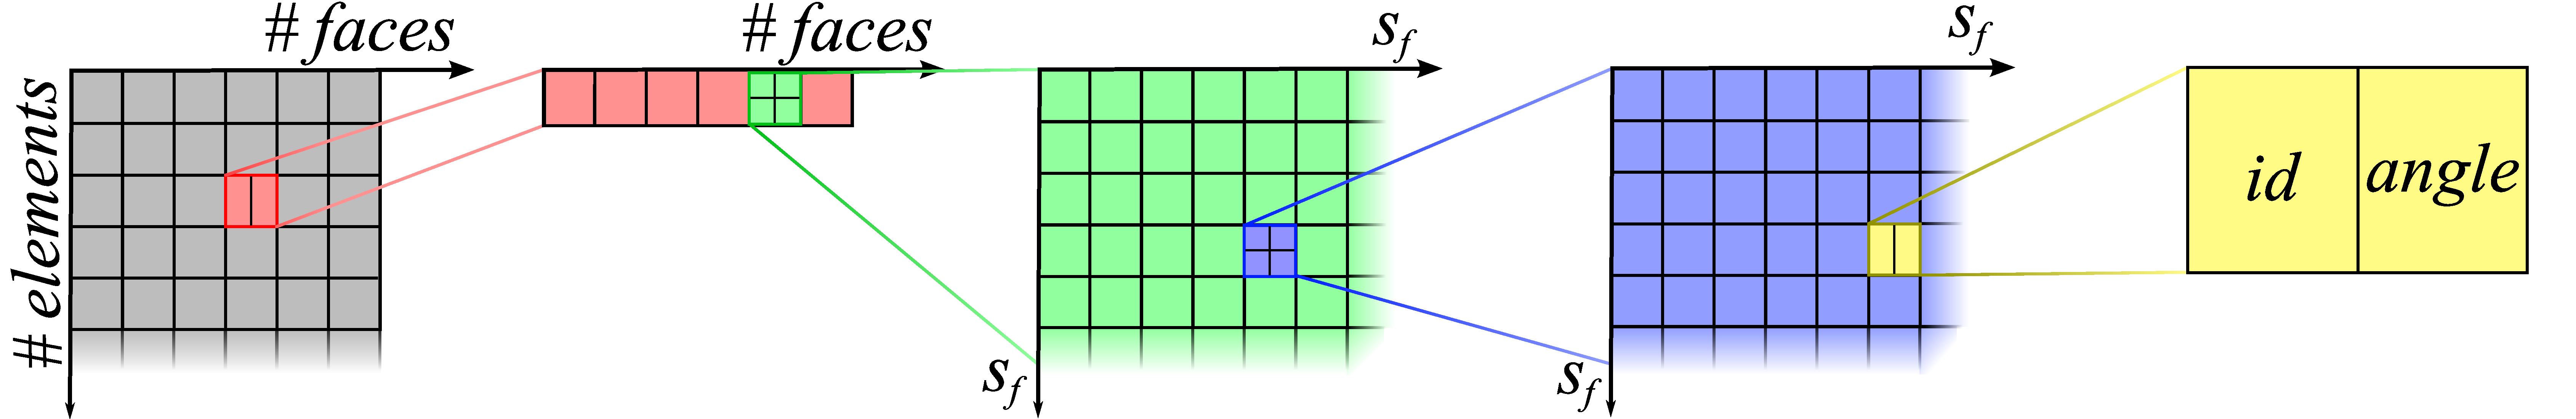
\includegraphics[width=0.75\linewidth]{figures/memory_layout.pdf}
    \caption{Memory layout used to gain access to the precomputed proxy ray information. To retrieve the information required during rendering in constant time, a hierarchical subdivision is used. For each proxy ray, we store the cluster ID as well as the rotation angle $\theta$.}
    \label{fig:memory_layout}
\end{figure*}
%
%
%
\subsection{Ray Interpolation}
In order to improve the image quality of our ray-casting approach, we introduce two specialized interpolation schemes: \emph{inter-ray interpolation} and \emph{intra-ray interpolation}. With the inter-ray interpolation we use the four nearest proxy rays  instead of the "nearest-neighbor" proxy ray for a given pixel position, and interpolate between them. This interpolation is carried out by using bilinear interpolation at every sample position along the viewing ray. The interpolation factors for these bilinear interpolations are based on the factors derived for the entry and the exit face. The intra-ray interpolation, instead, employs swapping of entry and exit points in order to obtain a mirrored copy of the current ray. Thus we can interpolate between the original ray at position $t$ and the mirrored ray at position $t'=1-t$ while traversing the initially obtained ray. Both of these interpolation schemes improve the image quality in situations where only a low resolution is available, as we show in Figure~\ref{fig:rayinterpolation}.
%
%
%
\section{Implementation}\label{sec:implementation}\label{subsec:limitations}
In this section, we explain all relevant implementational details regarding concepts  mentioned previously.

\noindent \textbf{Proxy Ray Generation.} %In order to get a suitable point distribution on the faces of the elements, we subdivide each element's face in the $\xi$ coordinate system. The points in $\xi$ space are transformed into world space by the formula presented in Section~\ref{sec:theory}. For each pair $(p_0, p_1)$ of entry- and exit-points, we compute the (in world space) straight ray between $p_0$ and $p_1$ and sample it in $s_r$ equidistant positions. Each sample point is transformed from world to $\xi$ space using an iterative Newton method and stored for use as one control point for the Catmull-Rom spline approximating the original ray. 

In order to have a consistent memory layout we will use the same data structure to store the computed control points here as we will use  later in the rendering stage. There are two demands on the data structure: given the parameters for the stored value, access should be in $O(1)$ and it should have a rectangular structure to be efficiently usable at GPU level. The parameters necessary for describing each proxy ray uniquely are $(e, f_s, f_e, p_s, p_e)$, with $e $ being the element number, $p_s$ the position on the entry face, $f_s$, and $p_e$ the position on the exit face, $f_e$. Let $\left|E\right|$ denote the total number of elements and $\left|F\right|$ be the number of faces per element. Furthermore, recall that $s_f'$ and $s_f''$, as defined in Section~\ref{subsec:proxyraygeneration}, are the subdivision parameters that control the number of points on the entry and exit face respectively. It then holds true that $p_f' \in [0,s_f']$ and $p_e \in [0,s_f'' - 1]$. Figure~\ref{fig:memory_layout} shows the memory layout that we have chosen for this setting. At the highest level of the hierarchy we arrange the data based on $f_s$ along the $x$-axis and $e$ along the $y$-axis. Thus we obtain $\left|F\right| \cdot \left|E\right|$ cells which contain the precomputed information for rays entering $e$ through $f_s$. Each of these cells is partitioned based on the $f_e$ along the $x$-axis, such that the resulting cells contain only the information for those rays exiting through $f_e$. We again partition the cells based on the number, $s_f'$, of precomputed points on the entry face. Finally the obtained cells are partitioned based on the number, $s_f''$, of precomputed points on the exit face. The memory layout depicted here is represented by the two following equations which allows us to store all data in a rectangular manner: 
\begin{eqnarray}
p_x &=& (f_s \cdot (s_f' \cdot s_f'' \cdot \left|E\right|)) +(f_e \cdot (s_f' \cdot s_f'')) + (p_{s,x} \cdot s_f'') + p_{e,x}\\
p_y &=& (e   \cdot (s_f' \cdot s_f'')) + (p_{s,y} \cdot s_f'') + p_{e,y}
\end{eqnarray}

\noindent \textbf{Curve Similarity.} The first step here is to increase the similarity of the stored proxy rays in such a way, that the subset, $R'$, is as small as possible. Three transformations are performed after which each proxy ray fulfills three traits. 1. The starting point, $x_0$, is at $(0,0,0)$. 2. The first non-colinear point $x_i$ lies in the $yz$-plane. 3. The end point, $x_n$, is at $(0,0,1)$. We apply three matrices $M_t$, $M_{rot}$, and $M_s$ to all control points, where $M_t$ is a translation by $-x_0$, $M_s$ is a scaling by $1 / (x_n.z)$, and $M_{rot}$ is a rigid-body transformation that will rotate the points such that $x_n$ is on the $z$ axis and the non-colinearity is fulfilled. The multiplication $M_s \cdot M_{rot} \cdot M_t$ is equal to $M_{trans}$ as mentioned previously. Thus we get new control points $x' = M_s \cdot M_{rot} \cdot M_t \cdot x$ with a higher degree of similarity between proxy rays. By enforcing that $x_i$ lies in the $yz$-plane we lose the rotational angle w.r.t. the z-axis. We will store this angle $\theta$ for each proxy ray separately so that we can access it together with the cluster id.

\noindent \textbf{Curve clustering.} In order to reduce the number of proxy rays which need to be stored on the graphics card, we apply a clustering algorithm such that multiple rays are represented by a single representative. Finding a good number of iterations for the applied K-means algorithm a priori is a hard problem, so we investigated multiple strategies. The simplest, and already feasible, strategy to use is a fixed number of iterations (see Figure~\ref{fig:clustering_epsilon_error}). Another possible solution is to trace the percentage of splines that change clusters in a single iteration, based on the assumption that this number decreases asymptotically to 0. A CPU implementation using C++ and OpenMP was used to generate the measurements presented in Section~\ref{sec:results}. The clustering was performed on 8 threads and it was found that the hard disk access, as well as the computing power, are bottle necks for faster execution times. Additionally, an OpenCL-based implementation was tested that keeps the cluster representatives for the current iteration in local memory and fetches the splines from global memory.

\noindent \textbf{Ray Marching.} The rendering step starts with a depth peeling step to get the entry- and exit points for each view ray. In general we set the additional depth test to accept all fragments which have a greater depth than or equal to that of the current fragment. To resolve the two coincidence cases, as presented in Section~\ref{subsec:peeling}, we ensure that each pair of entry- and exit-points has the same element ID. This, together with ensuring different face IDs, is enough to correctly resolve the point and the surface coincidence (see Figure~\ref{fig:depthcoincidence}). This additional information also leads to a more stable algorithm w.r.t. the available accuracy of the depth buffer. We tested depth buffer accuracies of 16 and 24 bits but found no noticeable visual differences. The approach also works for several situations where the entry and exit points lie on the same surface, as these points in general have unequal depth values thereby making the test for face inequality unnecessary. In the case of a silhouette edge, where two fragments coincide in the same depth value and originate from the same element, we do not perform a depth peeling but transform only the entry point and obtain a single sample.

The geometry representation of the FE models contains 4 values for each node; the three color channels provide the $\xi$ value (see Figures~\ref{fig:depthpeeling:entryxi} and \subref{fig:depthpeeling:exitxi}) and the alpha channel stores the element for which the nodal value is defined (see Figures~\ref{fig:depthpeeling:entryid} and \subref{fig:depthpeeling:exitid}). Based on this information, all free parameters for Equations 1 and 2 can be derived. Thus, the cluster can be fetched for this entry-exit point pair and the ray marching can be performed on the spline.

\noindent \textbf{Element Generalization.} The examples in this paper all use elements with cuboidal parent elements. In order to apply the technique to differently shaped elements, e.g., tetrahedral elements, methods must be implemented for depth peeling and sampling the element faces. This is straight forward. In fact, the current implementation already works for differently shaped elements, e.g. where multiple vertices of the parent element are mapped to the same vertex in world coordinates. This is the case for the apex of the left ventricular model, where the resulting elements have a curved wedge-like shape.  
%
\begin{figure}
    \centering 
    \subfigure[surface rendering]{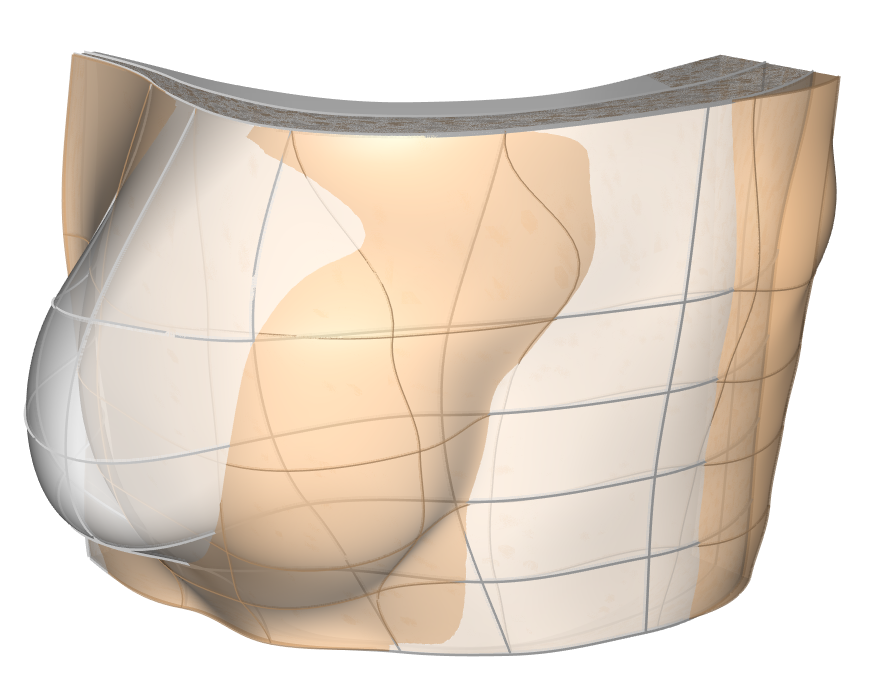
\includegraphics[width=0.4\linewidth]{figures/fem-breast}}
    \subfigure[volumetric rendering]{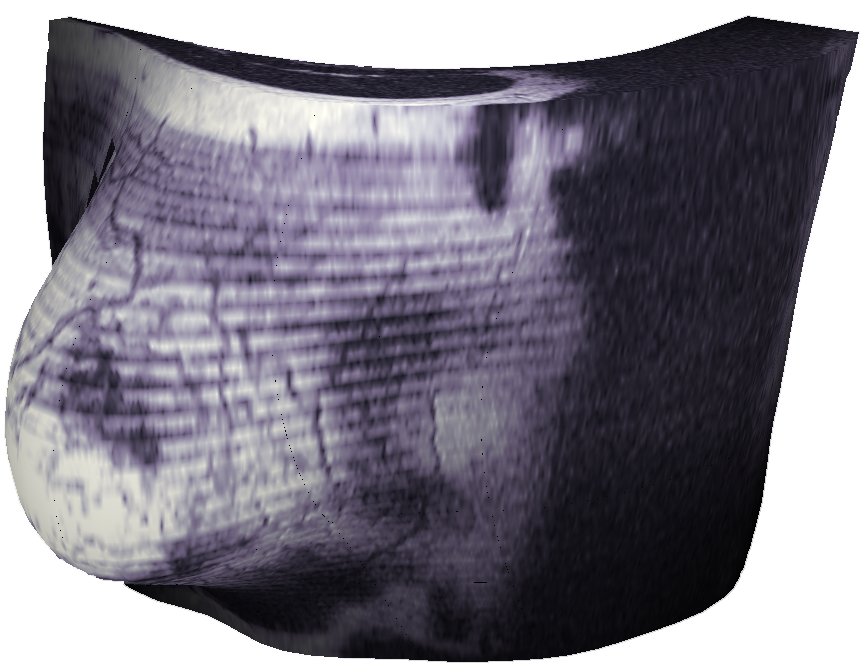
\includegraphics[width=0.4\linewidth]{figures/Breast}}
    \caption{FE breast model with MRI material space rendered as surface representation showing the deformed and the undeformed surface (a), and showing the deformed volume with our interactive volumetric approach (b).}
    \label{fig:breast}
\end{figure}
%
\begin{figure}
    \centering 
    \subfigure[polygonal rendering]{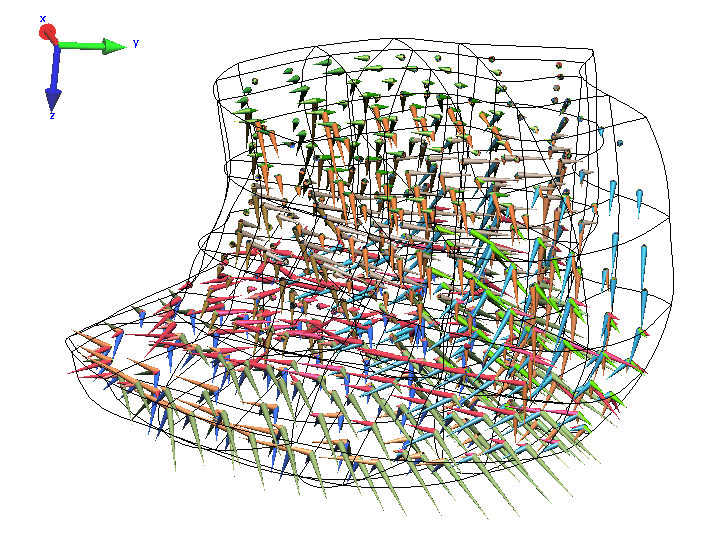
\includegraphics[width=0.42\linewidth]{figures/fem-tongue}}
    \subfigure[opaque volumetric rendering]{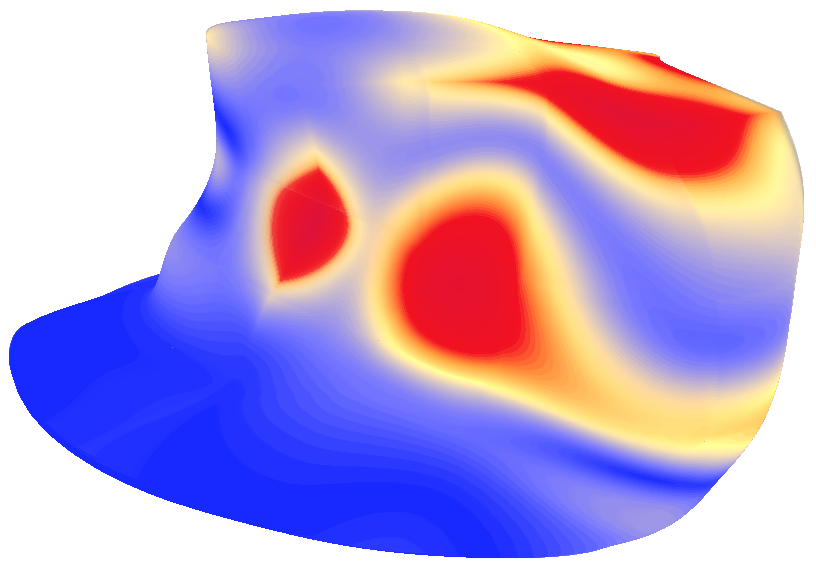
\includegraphics[width=0.42\linewidth]{figures/tongue3}}\\
    \subfigure[translucent volumetric rendering]{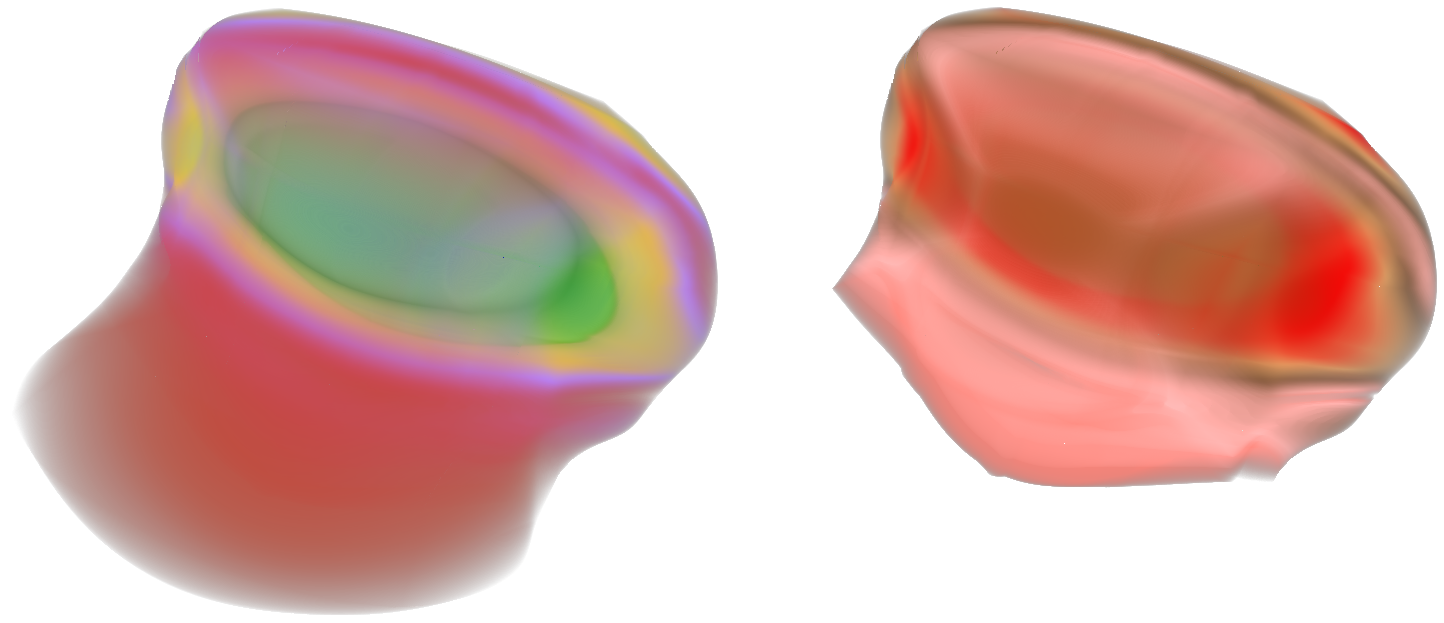
\includegraphics[width=0.84\linewidth]{figures/fem-tongue-new-sidebyside}}
    \caption{FE tongue model rendered as a polygonal representation, (a), and with our interactive volumetric approach, (b) and (c).}
    \label{fig:tongue}
\end{figure}
%
%
%
\section{Results}\label{sec:results}
To assess the quality and the performance of the proposed visualization technique we have applied it to different data sets. Below we discuss the visual results, the introduced errors and, the performance of our approach as well as the memory requirements.
%
%
%
\subsection{Visual Results}
To demonstrate the visual outcome of the proposed concepts, we have applied them to different FE models which all consist of elements with curvilinear boundaries. These vary with respect to the number of cells and the order of the used interpolation functions. Although we include only interpolation functions of a degree-7 or 9 polynomial, our method is not limited to any specific order as long as the coherencies are fulfilled. In the following paragraphs we describe these models and the visual results achieved.

\noindent \textbf{Breast model.} We have applied our approach to a deformation model of a breast data set, consisting of 60 tricubic elements, acquired from an MRI scan. The dependent variables in this case are the actual intensities of the MRI field, and the FE modeling has been applied to predict the supine shape of the data set originally acquired in the prone position. Figure~\ref{fig:breast} shows a comparison of the supine position rendered with our interactive volumetric approach, (b), as compared with a standard surface based representation, (a).

\noindent \textbf{Tongue model.} Furthermore we have applied our approach to a model of a human tongue, consisting of 64 tricubic elements, with simulated tissue densities and muscle fiber directions. In this case each node stores one coordinate vector, and seven derivatives and mixed derivatives for the tensor product of the cubic Hermite interpolation functions in all three coordinate directions. The results, as compared with a polygonal representation, are shown in Figure~\ref{fig:tongue}. In this case in particular, the multi-parametric capabilities of our algorithm are beneficial as the tongue model contains a relatively high number of parameters. When one would apply resampling to all of these parameter volumes instead, this would result in an unmanageable amount of data for a reasonable resolution.

\noindent \textbf{Heart model.} A heart data set, which consists of 16 bicubic-linear elements (i.e.~two interpolation functions are of cubic order, the other one is linear),  where the strain values for each point have been computed from displacements  obtained from tagged MRI data, serves as the third example (see Figure~\ref{fig:teaser}). For our visualization we have taken into account the three principal strain directions, which are the eigenvalues of the tensor. The principle strains include the maximum and minimum deformation and the corresponding eigenvectors give the direction of these deformations. These directions are circumferential, longitudinal and radial.
%
\begin{table}[b]
  \caption{Performance analysis (in fps) of our technique for different grid sizes compared with a straightforward (SF) implementation. The setups match the first three subfigures in Figure \ref{fig:teaser}: images showing radial strain, circumferential strain, and longitudinal strain.}
  \label{tab:performance}
  \begin{center}
    \begin{tabular}{|l|c|c|c|c|c|}
      \hline
      Figure \ref{fig:teaser} & Pixel & GPU & \multicolumn{3}{c|}{Our Technique [$s_f$, Clusters]}\\
      TF Setups & Res & (SF) & $3,1024$ & $5,2048$ & $10,4096$ \\
      \hline
      Radial & $256^2$ & 2.58 & 14.52 & 14.25 & 14.05\\
      Strain & $512^2$ & 1.33 & 11.40 & 11.71 & 11.02\\
      & $1024^2$ & 0.41 & 7.09 & 7.02 & 6.83\\
      \hline
      Circum- & $256^2$ & 2.60 & 14.63 & 14.81 & 14.21\\
      ferential & $512^2$ & 1.30 & 12.09 & 11.85 & 11.72\\
      Strain & $1024^2$ & 0.40 & 7.15 & 7.12 & 7.10\\
      \hline
      Longi- & $256^2$ & 2.53 & 14.66 & 14.70 & 14.74\\
      tudinal & $512^2$ & 1.35 & 11.78 & 11.78 & 11.83\\
      Strain & $1024^2$ & 0.40 & 7.12 & 7.12 & 6.88\\
      \hline
    \end{tabular}
  \end{center}
\end{table}
%
\begin{figure}
    \centering
    \subfigure[Straightforward approach]{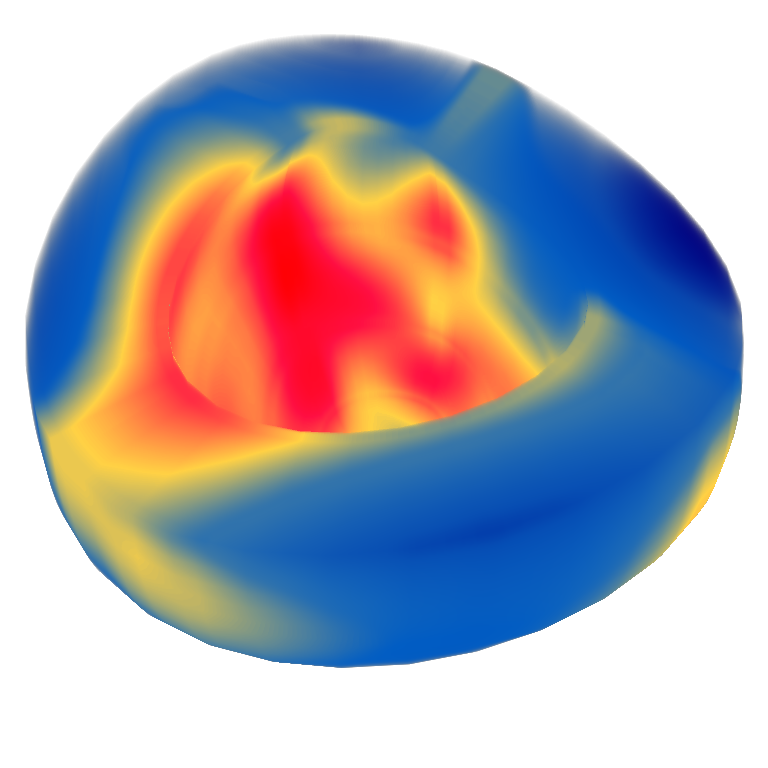
\includegraphics[width=0.32\linewidth]{figures/heart-comparison-straight-forward.png}}
    \subfigure[Our approach]{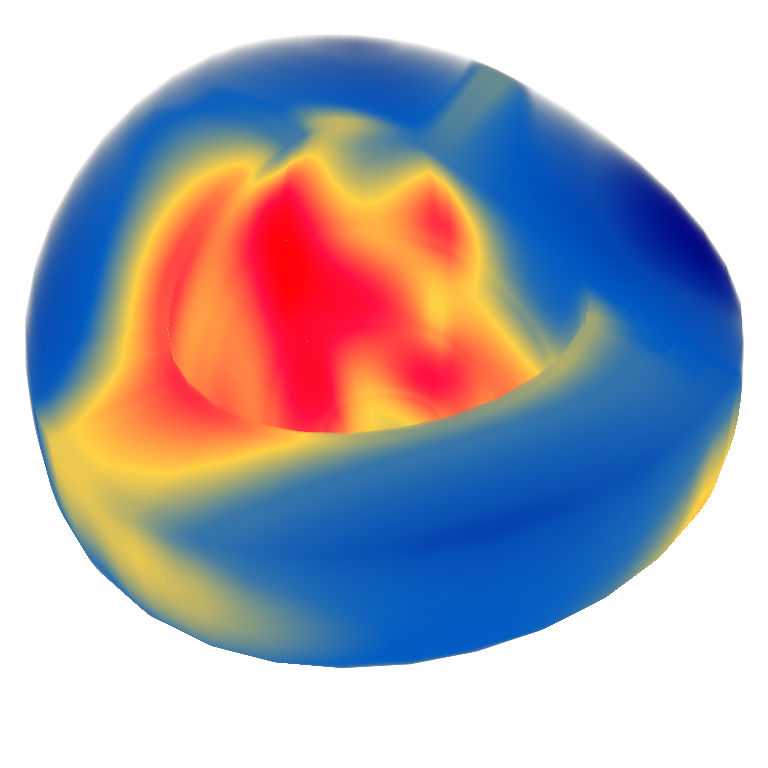
\includegraphics[width=0.32\linewidth]{figures/heart-comparison-clustering.png}}
    \subfigure[Visual difference (emphasized 10 times)]{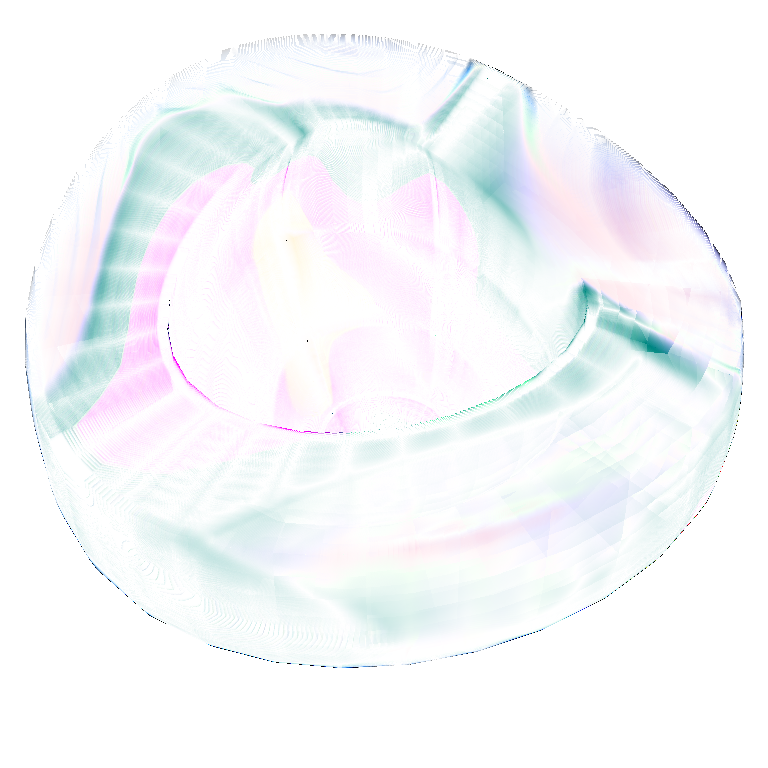
\includegraphics[width=0.32\linewidth]{figures/heart-comparison-diff-times-ten.png}}
    \caption{Visual error as obtained when applying our technique. A straightforward volumetric approach (a) and our interactive volumetric approach (b) have been compared, which results in the error image exaggerated tenfold (c).}
    \label{fig:heart-analysis}
\end{figure}
%
%
%
\subsection{Error Analysis}\label{subsec:error}
\begin{figure*}[t]
    \centering
    \subfigure[Error introduced by approximating the bent ray by a spline]{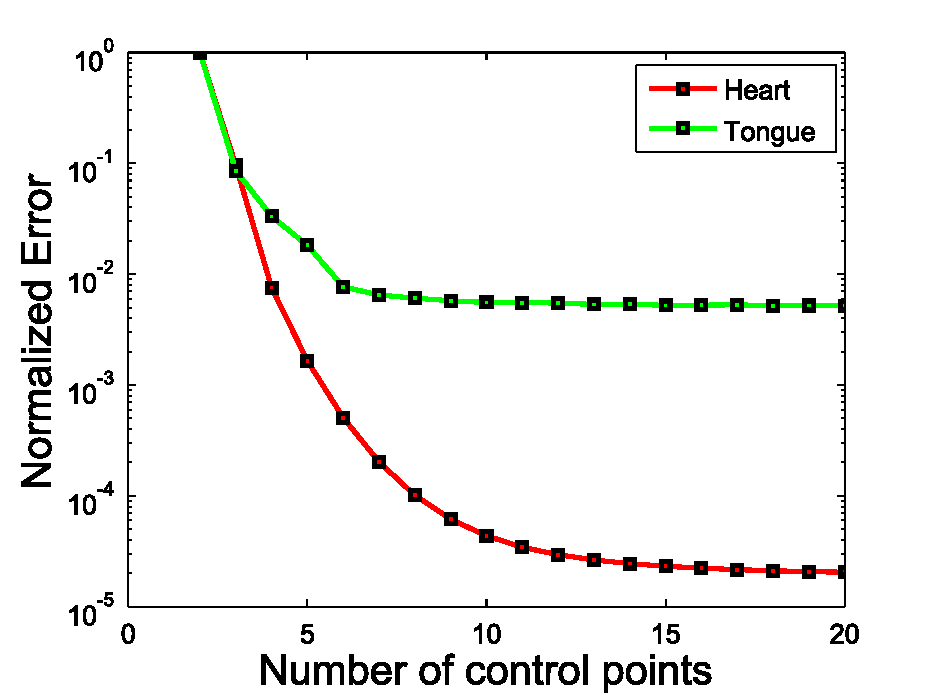
\includegraphics[width=0.325\linewidth]{measurements/spline_approximation/spline_approximation.pdf} \label{fig:spline_control_points_error}}
    \subfigure[Error introduced by clustering]{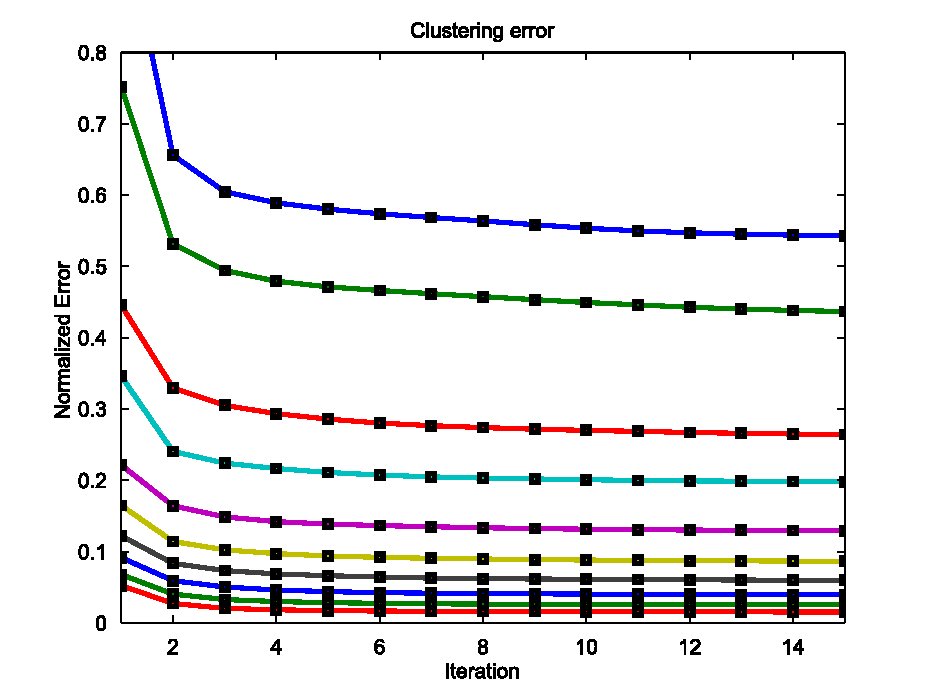
\includegraphics[width=0.325\linewidth]{measurements/clustering/clustering_error.pdf} \label{fig:clustering_epsilon_error}}
    \subfigure[Image error measured for varying cluster sizes]{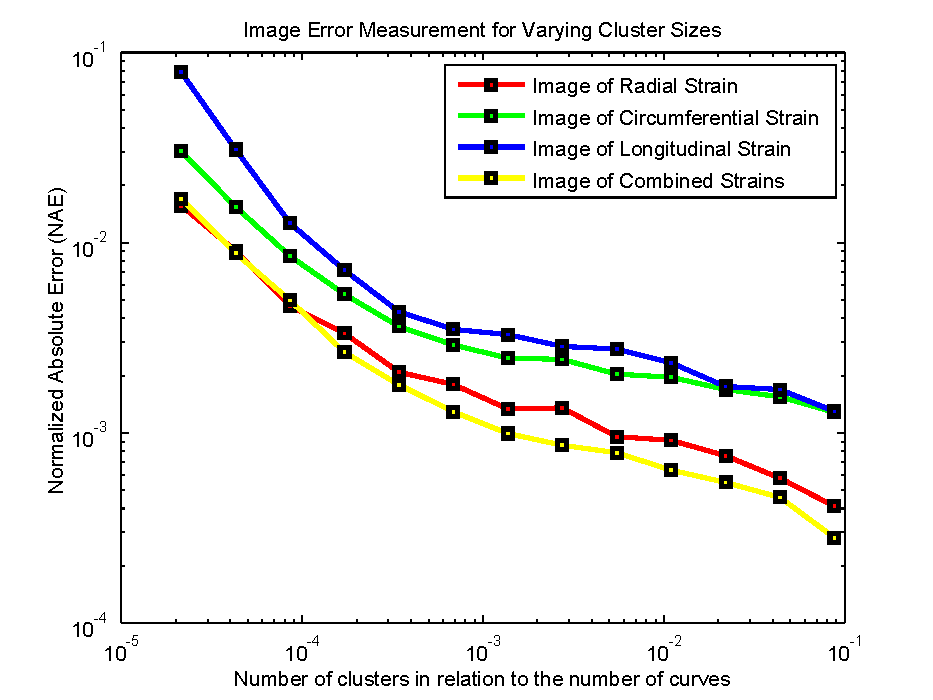
\includegraphics[width=0.325\linewidth]{measurements/cluster_measurements/clusterErrorPlot.pdf} \label{fig:clustering_visual_error}}

    \caption{\textbf{Error measurements.} \subref{fig:spline_control_points_error} shows the error introduced by the approximation of the correct bent ray by sampling a spline. The abscissa shows the number of control points used to construct the spline, where 2 points represent a straight line. \subref{fig:clustering_epsilon_error} shows the error for varying numbers of clusters depending on the number of iterations after which the k-means algorithm has stopped. Based on the heart data set with a grid resolution of $5\times5$, which resulted in 360.000 rays. \subref{fig:clustering_visual_error} shows the normalized absolute pixel error (background pixels are neglected) plotted against the percentage of clusters relative to the total amount of curves. The calculations have been performed on the subfigures of Figure~\ref{fig:teaser}, thus varying the transfer function and strain direction. All error values were normalized w.r.t the respective highest error.}
    \label{fig:error}
\end{figure*}

Our rendering approach contains several steps which potentially introduce visual errors. First, the proxy ray generation explained in Subsection~\ref{subsec:proxyraygeneration} introduces an error based on the number of actual proxy rays. The visual impact of this error is analyzed in Figure~\ref{fig:rayinterpolation}. In the two rows, different numbers of proxy rays have been computed. In the top row a very low number, with $2 \times 2$ proxy rays, per element face has been chosen whereas the bottom row uses $10 \times 10$ proxy rays. As can be seen, the error introduced by a low number of proxy rays is clearly visible. However, when using $10 \times 10$ proxy rays no artifacts are visible when using the proposed ray interpolation mechanism. As the clustering itself also introduces an error, we have analyzed the impact in Figure~\ref{fig:clustering_epsilon_error}, which shows the error for a varying number of clusters. It is obvious that the error becomes smaller if we use more clusters. The number of clusters can, depending on data set, be quite low in relation to the number of proxy rays as seen in Figure~\ref{fig:clustering_visual_error}. While these two analyses show the error for the proxy ray computation and the clustering separately, we have also compared the results achieved by our algorithm with the ground truth, a straightforward raycaster as described in Section~\ref{sec:preprocessing}, which evaluates the world-to-$\xi$ transformation during each sample step. We chose this method as a comparison, because it produces the smallest error by itself and is thereby suited to demonstrate the error introduced by our method. As can be seen in Figure~\ref{fig:heart-analysis}, the visual error is rather low, as only a tenfold exaggeration of the generated error image makes it noticeable.

We described in Section~\ref{subsec:proxyraygeneration} that we can use a varying number of control points to represent the proxy ray. This, of course, is an approximation of the original bent ray we get by using the straightforward implementation. Therefore we analyze the effect of this parameter has the error introduced by the representation. Figure~\ref{fig:spline_control_points_error} shows this error, computed by comparing the spline representation to the ray where each sample point is transformed. We sampled every ray at a sufficiently high rate of 1024 points and computed the area metric as described in Section~\ref{subsec:curvecompression}. The abscissa shows the number of control points representing the proxy ray, where 2 points denote a straight line. For easier comparison, all error values were normalized with respect to this value. As the error is dependent on the shape of the FE, we computed the error for all proxy rays in the \emph{Heart} and \emph{Tongue} models.

%\todo{Rewrite}
%Another source of error which is introduced into the pipeline is the tessellation of the curved elements. In order to perform the depth peeling, we need to represent the curved surfaces by piecewise-linear approximations. Although this results in an error on the final image, neither the speed nor the memory footprint of our method is affected by the tessellation of the curved elements.
%
%
%
\subsection{Performance Analysis}\label{subsec:performance}
\begin{table}[b]
  \caption{Memory consumption of data structures during rendering for varying grid resolutions and number of clusters on the heart dataset.}
  \label{tab:data_size}
  \begin{center}
    \begin{tabular}{|l|c|c|c|c|c|c|}
      \hline
      $s_f$ &  Without & \multicolumn{3}{c|}{With Certain Number of Clusters}\\
      	       & Clustering & 512 & 2048 & 4096\\
      \hline
      3	&	 2.7\,MB	&	0.39\,MB		&	0.47\,MB	&	0.82\,MB  \\
      8 	&	135\,MB	&	18\,MB		&	18.1\,MB	&	18.5\,MB	\\
      10 	&	329\,MB	&	43.9\,MB		&	44.0\,MB	&	44.1\,MB	\\
      15	&	1.62\,GB	&	222.5\,MB		&	222.6\,MB	&	222.9\,MB \\
      \hline
    \end{tabular}
  \end{center}
\end{table}

We have to differentiate between the precomputation and the rendering step in the performance analysis. Although the time used for precomputation is dependent on both the proxy ray computation and the clustering, the latter takes more time than the former. In our unoptimized CPU implementation, the clustering for a $5\times5$ proxy ray setup with $8192$ clusters takes roughly 4-6 hours, while a $15\times15$ setup with $8192$ clusters takes approximately 72-84 hours of time. We managed to reduce this time with an unoptimized OpenCL implementation by an order of magnitude to about 20-25 minutes for the $5\times5$ proxy ray setup with $8192$ clusters, which is in line with former works~\cite{mess10gpuclustering}. The clustering and all performance tests were executed on an Intel Xeon Quad-Core 3.06\,GHz with 6\,GB of working memory, equipped with a Geforce~580 card with 1\,GB of memory.

Table~\ref{tab:performance} shows the rendering performance of the presented volumetric FE visualization technique, as compared with the straightforward volumetric GPU implementation. As can be seen, the performance of our technique is affected by image resolution and independent of the number of clusters and proxy rays. The rendering quality is thus affected by a trade-off between the number of proxy rays used during the precomputation and the number of clusters used during the curve compression. In the worst case tested our technique provides above $7$\,fps instead of $0.4$\,fps. While the $14.81$\,fps achieved with our method in the best tested case enabled full interactivity, the $7$\,fps also resulted in an interactive experience.
%
%
%
\subsection{Memory Requirements}\label{subsec:memory}
A limiting factor of the presented method is the memory that is required to store the proxy rays, angles and cluster IDs. Besides the computational time, the available graphics memory is the only limitation to the number of elements, grid resolution, and number of clusters. In this section, we will consider the impact of each of these factors on the memory requirements using the same definitions as in Section~\ref{sec:implementation} with the addition of $c$ as the number of clusters. The total number of rays per element is given by $r_t = (s_f' \cdot s_f'' \cdot \left|F\right|)^2$ which leads to $e \cdot r_t \cdot s_r$ points that have to be transformed and stored. It should be noted that this data does not need to fit on the graphics card and is only an intermediate result. The required memory after the clustering has been performed can be estimated by: $c \cdot s_r + e \cdot r_t\cdot 2$. The first part of the equation is the storage necessary for the clustered control points of the representatives. The second part is the lookup table as described in Section~\ref{subsec:peeling} and needs to store both the cluster ID as well as the angle. A significant restriction on our method is obvious in the latter formula. The second term grows linearly in the number of elements and poses, therefore, a limitation on the mesh sizes we are able to render. Example values for the heart are given in Table~\ref{tab:data_size}, when we assume float precision, i.e., every point will occupy 12\,bytes of memory, and 5 stored points per cluster.
%
%
%
\section{Conclusions \& Future Work}\label{sec:conclusions}
In this paper we have presented a ray-casting based approach that enables the interactive exploration of high-order FE models. By shifting the computationally complex world-to-material transformation from the rendering stage into a preprocessing stage we are able to achieve interactive frame rates and thus allow for an interactive, in-detail, multi-parametric inspection of FE models using transfer functions and other parameters on standard GPUs. We have demonstrated the outcome of the presented approach by applying it to several real-world data sets and analyzing the errors introduced by our approach. Furthermore, we have discussed the rendering performance gain as well as the memory requirements.

There are several opportunities to further improve the presented concepts in the future. When precomputing the proxy rays we currently use a equidistant layout for the generation of the set, $P$, of uniformly distributed start and end points. In comparison with such an equidistant layout more elaborate sampling schemes, as used in many areas of computer graphics, might lead to an improved quality with the same number of proxy rays. While our approach currently supports scalar data only, in the future we plan to use the proposed method to display vector and tensor data defined over $\xi$ space.
%
%
%
\acknowledgments{We thank all reviewers for their fruitful comments which
helped to greatly improve this paper. We would also like to thank Prof.~Martyn Nash, Assoc.-Prof. Poul Nielsen, and Assoc.-Prof. Alistair Young, for providing the data sets we used in this work. This work was partly supported by grants from the Swedish Research Council (VR, grant 2011-4113), the Excellence Center at Link\"oping and Lund in Information Technology (ELLIIT) and the Swedish e-Science Research Centre (SeRC). The presented concepts have been realized using the Voreen open source visualization framework (www.voreen.org).}

\bibliographystyle{abbrv}
\bibliography{literature-fem}

\end{document}